%!TEX TS-program = xelatex
\documentclass[12pt]{./tex/thesis-umich}

\usepackage{acronym}
\usepackage{amsmath}
\usepackage{graphicx}
\usepackage{xcolor}
\usepackage{mathspec}
\usepackage{cite}
%\usepackage{xfrac}
%\usepackage{booktabs}
%\usepackage{listings}

\defaultfontfeatures{Mapping=tex-text, Ligatures={Common}}
\setmainfont{TeX Gyre Termes}
\setsansfont{TeX Gyre Heros}
\setmonofont{TeX Gyre Cursor}
\setmathfont(Digits,Latin,Greek){TeX Gyre Termes}

\title{Population Kinetics of a Repetitively-Pulsed Nanosecond Discharge}
\author{Benjamin T. Yee}
\department{Nuclear Engineering \& Radiological Sciences}
\year=2013

\frontpagestyle{1}

\dedication{ %
  I would like to dedicate this dissertation to someone else.
}

\acknowledgments[6]{ %
  Who is this?
}
\acknowledgmentswidth{0.8}

\preface[2]{ %
  This is a dissertation about something; I really hope it's good.
}

\committee{ %
  Associate Professor John E. Foster, Chair \\
  Doctor Edward V. Barnat, Sandia National Laboratories \\
  Doctor Isaiah M. Blankson, National Aeronautics and Space Administration \\
  Professor Augustus Evrard \\
  Professor Mark J. Kushner \\
}

\chair{John E. Foster}

\showlistofappendices

\abbreviations{ %
  \acro{rpnd}[\textsc{rpnd}]{repetitively-pulsed nanosecond discharge}
  \acro{dbd}[\textsc{dbd}]{dielectric-barrier discharge}
  \acro{app}[\textsc{app}]{atmospheric-pressure plasma}
  \acro{lte}[\textsc{lte}]{local thermodynamic equilibrium}
  \acro{vfp}[\textsc{vfp}]{Vlasov-Fokker-Planck}
  \acro{eedf}[\textsc{eedf}]{electron energy distribution function}
  \acro{fiw}[\textsc{fiw}]{fast ionization wave}
  \acro{las}[\textsc{las}]{laser-absorption spectroscopy}
  \acro{lif}[\textsc{lif}]{laser-induced fluorescence}
  \acro{lcif}[\textsc{lcif}]{laser collision-induced fluorescence}
}

\begin{document}
  \chapter{Introduction}\label{chp:intro}
    \section{Overview}

Historically, the study of atmospheric-pressure plasmas (\acs{app}'s) is
indistinguishable from the study of plasmas as a whole. However, the detail of
the measurements and calculations associated with \acs{app}'s has been limited
by their complexity. From a computational perspective, the high pressure and
number of potential reactions present a difficult challenge. Likewise, the high
pressure can significantly complicate the data analysis for a number of plasma
diagnostics. Aside from the high pressures, the large electric fields, short
time scales, and general randomness of \acs{app}'s make even the most basic
observations a feat.

In the last several decades, some of this has begun to change. High-powered
computing has allowed simulations with remarkable detail. Similarly, advances in
technology has enabled plasma diagnostics in regimes that were experimentally
inaccessible. As a result, the body of knowledge regarding \acs{app}'s has
greatly increased. Sometimes, the motivation for this work is scientific
curiosity. More often, the study of \acs{app}'s has been driven by a broad range
of applications.

Among the first plasma applications were provided by \acs{app}'s: ozone
generation and lighting. Aside from these items, plasma welding, polymer
treatment, combustion, and plasma televisions have become widely accepted.
Meanwhile, a large number of new applications may soon be added to this list,
including: treatment of tissue wounds, altering airflow over airfoils, and
destruction of industrial pollutants.

Unsurprisingly, each case demands a different kind of plasma. The original arc
discharges were created between two graphite rods connected to immense battery
banks. In contrast, a modern research reactor studying plasma-assisted
combustion might use a fast-switching semiconductor circuit. Over the years,
several types of \acs{app}s have been developed for a variety of situations:
dielectric-barrier, corona, thermal arc, RF, microwave, pulsed, and more.

Within this group\footnote{The interested reader is referred to Starikovskaia's
review \cite{Starikovskaia2006} which provides a general overview of \acs{app}'s
in the context of plasma-assisted combustion}, the repetitively-pulsed
nanosecond discharge (\acs{rpnd}) has created considerable interest. Generally
speaking, a \acs{rpnd} is a plasma generated by a repetitive electrical pulse
applied between two electrodes. The pulse voltage is often in excess of one
kilovolt, lasts anywhere from $<1-100$ ns, and is repeated over a thousand
times each second. The result is a wave of ionization (and light) which crosses
from the powered electrode to the grounded one.

A \acs{rpnd} can fill volumes of several liters with a relatively uniform
plasma. Though they can cause significant excitation of the background gas, they
generally produce very little heating (in some cases below a detection limit of
$\Delta \pm 15$ K). In addition, the excitation can be changed with adjustments
to the magnitude or duration of the electrical pulse. Each of these
characteristics are highly desirable in one or more of potential applications
for \acs{app}'s.

Given all of these promising properties, \acs{rpnd}'s have been the subject of
substantial study by several research groups. However, much of this work has
focused on the physics of \acs{rpnd}'s in air. Unfortunately, air's large number
of constituent elements can lead to notable complexity. In turn, this can
obscure some of the more fundamental questions relation to \acs{rpnd}'s: how do
they form, how is the energy distributed between excited particles, and what
kind of spatial variation can be expected?

This paper details a study of each of these questions in a helium \acs{rpnd}.
Specifically, the densities of one particular excited atom are measured for a
variety of pressures and locations. This is complemented by measurements of the
light emissions for the same set of parameters. A simple model of a \acs{rpnd}
is used to predict several characteristics of the plasma based on the excited
state densities: electron density, electric field, and light emission. The
measured light emissions are interpreted to show how the energy is distributed
in the gas, and how it changes over time. Finally, they are compared with the
estimated light emissions to check the validity of several common assumptions.

\section{Literature Review}

\acs{rpnd}'s are only a recent invention which resulted from advances in
fast-switching semiconductors. However, the physics of their formation is
related to a much larger category of plasmas which includes lightning, sparks,
and even some transient phenomena in DC glows. These plasmas are unique in that
their formation occurs on timescales much faster than the traditional Townsend
mechanism allows for. The means by which these plasmas form has acquired several
names in the literature; here we will adopt the term, fast ionization wave
(\acs{fiw}).\footnote{It should be noted that the phrase wave does not indicate
any kind of periodic motion or spatial arrangement. Simply put, it describes a
boundary which separates ionized and unionized gas which travels from one
electrode to another.}.

\subsection{Early History of Pulsed Discharges}

The first \acs{fiw} was likely generated by Wheatstone in 1835
\cite{Wheatstone1835}. As reported by Thomson \cite{Thomson1893}, Wheatstone
built a vacuum tube six feet in length, and applied a high voltage across the
gas. As a plasma formed in the tube, Wheatstone observed its formation with a
rotating mirror. The use of this apparatus allowed Wheatstone to place a lower
limit on the speed with which the plasma travelled from one electrode to the
other. Though the discharge crossed the tube with a speed of at least
$8\times10^7$ cm/s, spectral observations indicated that the particles emitting
the light were not travelling at that speed \cite{Zahn1879}.

Later, Thomson revisited this work with an improved apparatus
\cite{Thomson1893}. This included a tube that was now 15 m in length and five mm
in diameter, as seen in figure \ref{fig:thomson}.
\begin{figure}
  \centering
  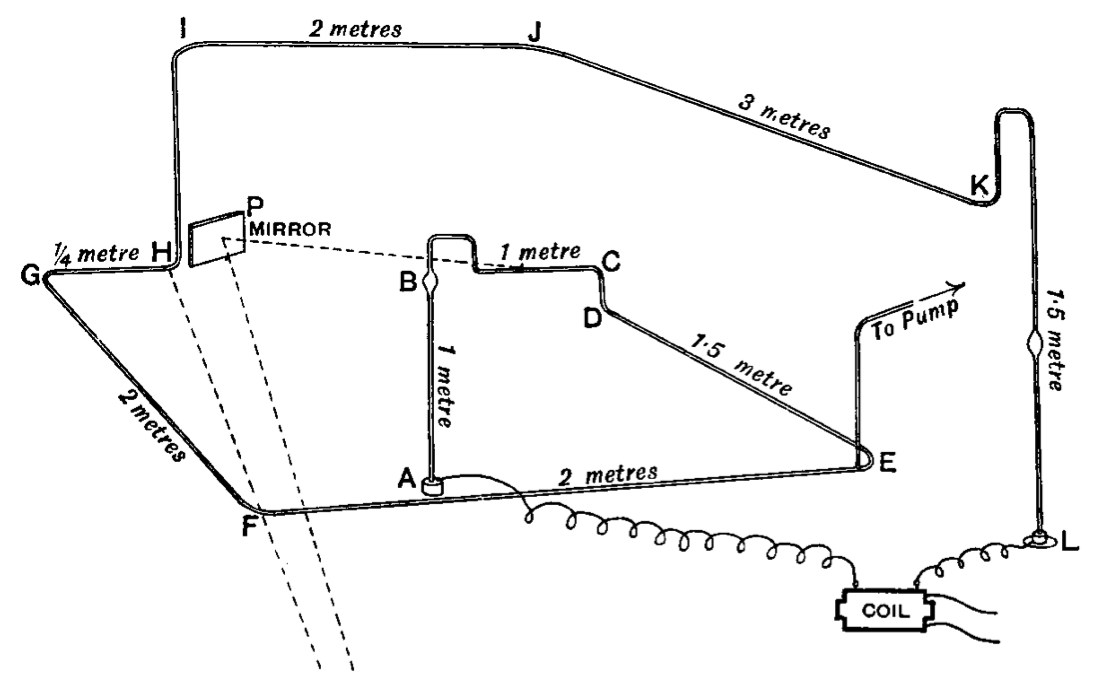
\includegraphics[width=4in]{chapters/introduction/figures/thomson.png}
  \caption{A sketch of J.J. Thomson's early experiments on fast ionization
  waves in long vacuum tubes.}\label{fig:thomson}
\end{figure}
Also using the rotating mirror apparatus, Thomson was able to greatly improve on
the estimates of Wheatstone. He estimated that the so-called ``luminous front''
had a speed that was more than $1.5\times10^{10}$, or in excess of half of the
speed of light. Furthermore, Thomson determined that the front always appeared
to travel from the positively pulsed electrode (anode) to the ground electrode
(cathode).

The study of these luminous fronts was revisited by several researchers in the
wake of Thomson \cite{James1904, Whiddington1925, Beams1926} with varied
success. By his own admission, Beams's work in 1926 was done ``hurriedly,''
using a rudimentary Kerr cell. In 1930, Beams returned to the propagation of
light pulses in vacuum tubes with a rotating mirror apparatus \cite{Beams1930}.
In addition to confirming his previous measurements, and those of Thomson, Beams
discovered that the \acs{fiw} always traveled from the electrode with the
highest absolute potential, to the lowest one. In other words, the wave could be
anode or cathode directed, depending on the magnitude of their potentials
relative to ground. Benefiting from an improved understanding of electricity,
namely the existence of electrons and ions, Beams was able to provide the first
hypothesis on the nature of the \acs{fiw}:
\begin{quote}
  In the neighborhood of the electrode $\ldots{}$ the field is very high and
  intense ionization should take place. This ionization due to the large
  difference in mobilities of positive ions, negative ions and electrons
  respectively should result in the establishment of a space charge. This space
  charge, once formed near the high potential electrode $Q$ must move down the
  tube regardless of the polarity of the applied potential because of the
  changes it produces in the field near its edges.
\end{quote}

At about the same time, Schonland and Collens reported on their observations of
lightning \cite{Schonland1933}. Though the general structure and length scale of
lightning is substantially different from the luminous fronts observed by Beams
and Thomson, the two phenomena would later prove to be very similar. In their
work Schonland and Collens noted that lightning would usually occur in a
two-step process. Based on the images they obtained, they suggested that
the leader was generated by a relatively small ``dart'' with a mean vertical
velocity of $7.2\times10^8$ cm/s. The dart moved in a random manner, changing
directions at random intervals, but always moving downward.

The second step began when this dart reached the ground. Once there, a bright
return stroke would occur along the same path that the leader had traced out. In
contrast to the leader stroke, the return stroke had a velocity of $5\times10^9$
cm/s. Schonland and Collens hesitantly attributed the leader stroke to an
extended electron avalanche, and the return stroke to thermal ionization along
the conductive path generated by the dart. However, calculations by Cravath and
Loeb showed that the speeds of the proposed avalanche would have to be
inconsistent with the fields at the head of a lightning stroke
\cite{Cravath1935}. Instead, they suggested that the dart was actually a moving
region of space charge which locally accelerated electrons to ionizing energies.
This was fundamentally similar to the mechanism proposed by Beams in 1930.

\subsection{The Streamer Model}

It was long known that sparks in air were similar to lightning. Advances in
technology during the 1930's led to experiments which reinforced this
similarity. In response to the measurements of Schonland and Collens; Snoddy,
Beams, and Dietrich studied the breakdown of gas in a long tube with an
oscillograph \cite{Snoddy1936}. The results from the oscillograph showed a very
clear return wave for which they measured several parameters the characterized
as a function of pressure and applied potential. They observed that at low
voltages, the system behaved like a large resistor in series with a capacitor,
and below a critical voltage, no return stroke would form. Finally, in order to
explain the propagation of the \acs{fiw} generated by the positive pulse, they
suggested that photoionization was occurring in the space ahead of the wave.

Around the same time, Flegler and Raether had come to a similar conclusion,
leading to the first attempt at a theory describing streamers
\cite{Flegler1936}. This same theory was proposed independently by Loeb and Meek
in a series of papers \cite{Loeb1940, Loeb1940a, Meek1940}. The streamer theory
divided the initial breakdown of a spark into two steps. In the first step, an
electron avalanche is initiated between two electrodes. The avalanche travels
toward the anode and leaves behind a region of high positive space charge. In
the second step, the return stroke begins at the cathode and travels toward the
cathode. It was suggested that the head of the return stroke ionizes the gas
ahead of it by pulling in background electrons or via photoionization.
\footnote{These early works emphasized the importance of photoionization. It is
now know that it is only required for cathode-directed streamers in systems with
no background ionization. In addition, Mesyats later showed that the lifetime of
the excited states responsible for photoionization were often longer than the
lifetime of the streamers \cite{Mesyats1972}}.

The streamer model proved relatively successful in describing the development of
sparks and lightning. Theoretical estimates of the speed matched the velocity
measurements that were acquired through photographs and oscillographs.
Additionally, the theory is able to account for the halting manner in which
lightning is formed, though it is only tentatively able to describe the
branching and stepped appearance. Finally, the streamer mechanism provides an
adequate explanation of why streamer discharges are not affected by the shape or
material of the cathode, namely, they do not depend on secondary electron
emission.

The study of the formation of streamers and lightning continues to be active to
this day. Following the initial work of Flegler, Raether, Loeb, and Meek, a
number of researchers began to explore the boundary between the Townsend
mechanism and the streamer mechanism. Most notable was Fisher and Bederson's
work in 1951 \cite{Fisher1951}, which was later extended to nitrogen
\cite{Kachickas1952} and argon \cite{Kachickas1953}. However, there were still a
number of phenomena that were poorly explained by the streamer model. In
particular, Kunhardt provided a useful overview of the problems in 1980
\cite{Kunhardt1980}. However, even before that, it was apparent that the
transients of sparks and lightning was more complicated than thought.

\subsection{Ionizing Waves of Potential Gradient}

Per Chalmers \cite{Chalmers1971}, Rogowski and Buss \cite{Rogowski1927,
Buss1932} observed a fast, diffuse, glow discharge immediately prior to the
filaments which often accompany a streamer discharge. Allibone and Meek, noted
similar diffuse discharges in air based on oscillographs and photographs
\cite{Allibone1938, Allibone1938b, Allibone1938c}. However, the Boys apparatus
which was employed in these studies (an ancestor to the modern streak camera)
was unable to capture the evolution of the diffuse glow, given its large spatial
extent.

This was first noted by Allibone who attempted to use Lichtenberg
figures\footnote{Such figures directly exposed photographic emulsions to the
electrical discharge. The developed image was a time-integrated representation
of the discharge.} to definitively capture this diffuse glow
\cite{Allibone1948}. Later, Saxe and Meek used the recently invented
photomultiplier tube to record the evolution of the light emissions in the
brief, diffuse glow \cite{Saxe1948} as a function of space. Both studies
agreed in the existence of the diffuse glow, despite some disagreement on the
nature of its geometry and propagation.

The similarity of fast transient ionization waves in certain glow discharges
\cite{Westberg1959} to those observed in lightning and streamers led Loeb to to
the conclusion that they were all the same phenomena \cite{Loeb1965}. He
referred to them as ``ionizing waves of potential gradient,'' as the proposed
mechanism for the waves was the generation of a steep potential gradient in a
sufficient short period of time. 

As reported by Babich, Loika, and Tarasova \cite{Babich1977}, the detection of
x-ray emissions from pulsed, high-pressure, helium discharges created a new
avenue of interest for these transient plasmas \cite{Stankevich1967,
Noggle1968}. Unlike the streamers, which were often filamentary, these new
discharges exhibited surprising uniformity. The primary difference being the
duration of the pulse (on the order of nanoseconds) and the applied potentials
(in excess of 200 kV).

The x-rays suggested that electrons in these discharges were accelerated to
unusually high energies (on the order of 10 keV) despite the high
collisionality. It was then that Babich and Stankevich suggested that the x-rays
resulted from continually accelerated electrons impinging on the metal
electrodes \cite{Babich1973}. Briefly, the electric fields in the fronts of the
ionizing waves were so large that they managed to accelerate electrons past the
peak in their collisional cross sections.

Mesyats, Bychov, and Kremnev attempted to provide a more rigorous explanation
for the uniform nature of these new discharges \cite{Mesyats1972}. After
conducting several experiments, they came to the conclusion that these transient
plasmas were the result of many overlapping avalanches, unlike the streamer
which only involves a single avalanche. Kunhardt and Byszewski later
expanded on this work by developing a kinetic model to explain the behavior of
all pulsed discharges above the Townsend threshold \cite{Kunhardt1980}.

It was based on the studies of the fast electrons in these discharges that
Mesyats, Bychov, and Kremnev proposed the use of a fast electron beam for
pumping high-pressure gas lasers. Similar work was conducted simultaneously by
Fenstermacher et al.~\cite{Fenstermacher1972}. Palmer \cite{Palmer1974}, and
Levatter and Lin \cite{Levatter1980} determined that there was a threshold
amount of preionization required to ensure homogeneity of the discharge. Hunter
\cite{Hunter1976}, and Koval'chuk and Mesyats \cite{Koval'chuk1976} later
proposed that such discharges be used for fast-closing switches. Gas lasers and
fast switches would drive much of the later research on fast, pulsed discharges.

Eventually these discharges came to be referred to as fast ionization waves
(\acs{fiw}s). A large body of Russian literature developed around their study,
though much of it has remained untranslated. In 1994, Vasilyak produced an
extensive review of these studies \cite{Vasilyak1994}. The data include wave
velocities for a variety of gases and pressures. Other parameters such as
attenuation coefficients for the waves, high energy electron currents, electric
field measurements, and a circuit model of the \acs{fiw} are also included.

\subsection{\textsc{rpnd}s}

Beginning in 1998, the Moscow Institute of Physics and Technology (\acs{mipt})
produced a flurry of studies on the \acs{fiw} \cite{Anikin1998, Pancheshnyi1998,
Starikovskaia1998}. They employed several different diagnostic techniques
(photomultiplier tubes and capacitive probes) in an exceptionally detailed study
in both air and nitrogen, using a shock tube and a bell jar. A summary of these
investigations can be found in \cite{Starikovskaia2001}. The work showed
exceptionally reproducibility of the discharge parameters at relatively low
repetition rates, on the order of tens of Hz, and evidence of runaway electrons.
This work also included some of the first approximations of the electron energy
distribution function (\acs{eedf}).

Interestingly, later analysis of a anode-directed \acs{fiw} in nitrogen by the
group at \acs{mipt} \cite{Pancheshnyi1999} concluded that the, the vast majority
of the electrons were generated \emph{after} the wave. This suggests that the
ionization in an \acs{fiw} does not strictly track the luminous front of the
wave. Additionally, measurements of the conductivity suggested that the local
approximation becomes invalid in the wave front and the electron energy
distribution function resembles a beam.

In 1997 the invention of the fast ionization dynistor (\acs{fid}) was revealed
\cite{Efanov1997}. These new devices enabled sub-nanosecond switching of 10's of
kilovolts, with repetition rates approaching 100 kilohertz. This was a leap
forward over previous technologies which generally used thyristors or spark gaps
for switching. Particularly appealing was the high repetition rate of the
\acs{fid}.

Recall that the volume-filling \acs{fiw} required a significant
amount of preionization. This was often accomplished an ionization source in
addition to the high voltage pulse (in the form of UV radiation, or electron
beams). However, the repetition rates of \acs{fid}s were high enough such that a
substantial number of electrons would carry over between pulses. These seed
electrons obviated the need for a preionization. In addition, the time-averaged
densities of excited states could maintained at much higher values. This had
particular promise for processing applications.

In the eventual commercialization of the \acs{fid} made economically feasible to
create fast, repeatable fast ionization waves. It is this class of discharges
which are now referred to as repetitively-pulsed nanosecond discharges, or
\acs{rpnd}s. Their uniformity, low gas heating, high-pressure operation, and
efficient ionization made them attractive or a number of applications:
\begin{itemize}
  \item plasma-assisted combustion \cite{Starikovskaia2006},
  \item magneto-hydrodynamic energy bypass \cite{Macheret2002},
  \item plasma actuators \cite{Adamovich2009},
  \item and high-pressure xenon lamps \cite{Nikandrov2008, Tsendin2009}.
\end{itemize}

As with the \acs{fiw}s, the primary diagnostics were current and voltage
characteristics, electric field measurements with capacitive probes, and
emission measurements with photomultiplier tubes. Later, intensified \acs{ccd}s
were used to record the emissions of specific transitions as well as broadband
light. This approach has been used to more clearly illustrate the uniformity and
reproducibility of the discharge \cite{Adamovich2009}. Other researchers have
turned to laser-based diagnostics, such as coherent anti-Stokes Raman
scattering, to measure gas heating \cite{Zuzeek2010} and the electric field in
molecular systems \cite{Ito2010, Ito2010a}. Likewise, laser collision-induced
fluorescence (\acs{lcif}) has been used to obtain axial profiles of excited
state and electron densities in helium \acs{rpnd}s \cite{Weatherford2012}.

Concurrent with these improvements in experimental techniques has been similar
progress in the simulation of \textsc{rpnd}s. The one-dimensional models 


  
  \chapter{Theory}\label{chp:theory}
    In order to properly understand the \acs{rpnd}--the experimental measurements,
and the models, it is necessary to develop a theoretical underpinning. The
\acs{rpnd} is an ionized gas, and, dependent on its characteristics, a plasma.
Therefore, we begin with a review of the statistical description of an ionized
gas, equilibrium solutions, and several approximations. Subsequently, the
discharge initiation process is considered from the perspective of a single
avalanche. The Townsend model is briefly reviewed, followed by a more detailed
explanation of the streamer model. This naturally leads to the development of a
homogeneous discharge condition based on the preionization density--the basis
for the \acs{rpnd}. Following this, a qualitative introduction to atomic
structure is provided in order to introduce spectroscopic concepts such as
energy levels, transitions, lineshapes, and absorption cross sections.

\section{Ionized Gas}
An ionized gas is a volume of gas in which some fraction of the neutral atoms
and/or molecules have been separated into electron and ion pairs. For a
sufficiently large number of particles and collision rate, the behavior of each
species in the ionized gas can be described by a continuous distribution
function.

This function is an expression of the likelihood of finding a particle within a
specific range of velocities in a specific volume, as a function of time. This
function is denoted as $f_\alpha(\vec{r}, \vec{v}, t)$, where the subscript
$\alpha$ denotes the species, $f$ is the distribution function, $\vec{r}$ is the
position, $\vec{v}$ is the velocity, and $t$ is the time.

The behavior of $f_\alpha$ can be shown \cite{Bellan2008} to be governed by the
Boltzmann equation,
\begin{equation}\label{eq:boltzmann}
  \frac{\partial f_\alpha}{\partial t} + \vec{v}\cdot\nabla f_\alpha +
  \frac{q_\alpha}{m_\alpha} \left(\vec{E} + \vec{v}\times\vec{B}\right)
  \cdot \nabla_v f_\alpha = \left( \frac{\partial f_\alpha}
  {\partial t}\right)_\mathrm{coll}.
\end{equation}
Here, $m$ is the particle mass, $q$ is its charg:, $\vec{E}$ is the electric
field, $\vec{B}$ is the magnetic field, and $(\partial f_\alpha/\partial
t)_\mathrm{coll}$ is a term which represents changes to the distribution
function as a result of collisions. Coupled with Maxwell's equations,
equation~\ref{eq:boltzmann} provides a complete description of the behavior of
the fields and particles in a plasma.

For a species in equilibrium in the absence of external forces and ($\partial
f_\alpha/\partial t)_\mathrm{coll} = 0$, it can be shown \cite{Druyvesteyn1940}
that the distribution of energies is
\begin{equation}\label{eq:mb}
  f\alpha(\epsilon) = C \epsilon^{1/2}
          \exp\left( -\frac{\epsilon}{\kB T_\alpha}\right)
\end{equation}
where $C$ is a normalizing constant, $\epsilon$ is the energy, $\kB$ is
Boltzmann's constant, and $T_\alpha$ is the temperature of the species. This is
referred to as the Maxwell-Boltzmann distribution. It should be emphasized that
this solution only applies when the classical species can be considered to be in
equilibrium. Gradients and electromagnetic fields can both significantly alter
the distribution function of a species. This can be of particular importance in
the calculation or reaction rates, or the measurement of temperatures.

Additionally, the Boltzmann equation may be solved for electrons in equilibrium
constant electric field, provided that a constant current density, and only
elastic collisions. This is generally valid if the electric field strength is
sufficiently small such that the mean energy of the electrons does not become
comparable to the threshold energies for inelastic collisions. This result was
originally presented by Druyvesteyn and Penning \cite{Druyvesteyn1940} and has
come to be known as the Druyvesteyn distribution. It is defined as,
\begin{equation}
  f_\alpha(\epsilon) = C \epsilon^{1/2}
           \exp\left(-\frac{\epsilon^2}{\langle \epsilon \rangle^2} \right)
  \label{eq:druy}
\end{equation}
where $\langle\epsilon\rangle$ is some mean energy, determined by the gas
properties. This solution tends to suppress the probability of higher and
lower-energy electrons in favor of more intermediate values.
Figure~\ref{fig:simpledists}
\begin{figure}
  \centering
  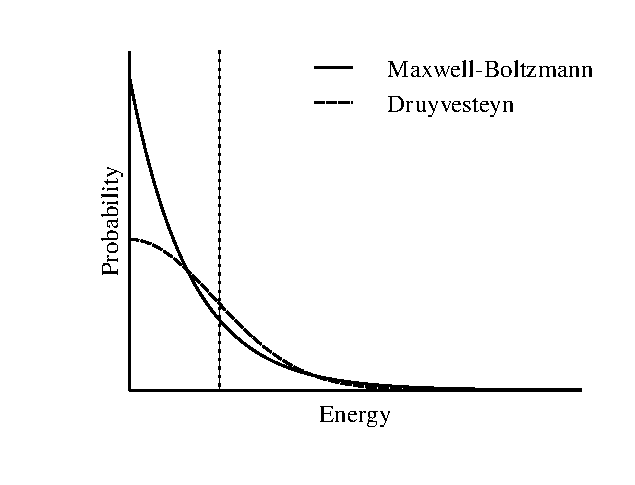
\includegraphics{./chapters/theory/figures/simpledists.eps}
  \caption{Comparison of the Maxwell-Boltzmann energy distribution and the
    Druyvesteyn distribution for the same average energy (illustrated by the
  dotted line).}
  \label{fig:simpledists}
\end{figure}
compares the probability distributions from equations~\ref{eq:mb}
a]nd~\ref{eq:druy} for the same temperature $T_\alpha$. The dotted line
illustrates the average energy for the two distributions, which is not the same
as the most probably energy.

Additional solutions of equation~\ref{eq:boltzmann} in anything but these simple
cases can be very challenging (c.f.\ chapter 18 of \cite{Lieberman2005}). Even
computational approaches can be stymied by the seven-dimension phase space and
high dynamic range. In most situations, the Boltzmann equation is reduced to
more tenable expressions by integrating over velocity-space (leaving $f$ as a
function of space and time). The first so-called moment is the conservation
equation or continuity equation \cite{Lieberman2005},
\begin{equation}\label{eq:cont}
  \frac{\partial n_\alpha}{\partial t} + \nabla \cdot (n_\alpha \vec{u_\alpha})
  = G_\alpha - L_\alpha.
\end{equation}
In this case, there is now a mean velocity $\vec{u}$, as well as gain ($G$) and
loss ($L$) terms which replace the collision operator. The gain and loss terms
are generally expressed as the product of the densities of the interacting
species, and a rate coefficient. For an electron-impact interaction where the
target is relatively stationary, the rate coefficient is
\begin{equation}
  K = \int_0^\infty f_e(\epsilon)\sigma(\epsilon)
      \sqrt{\frac{2\epsilon}{m_e}}d\epsilon,
\end{equation}
where $\sigma$ is the energy-dependent cross section.

The definition of the mean velocity, $\vec{u}$ can be obtained by multiplying
equation~\ref{eq:boltzmann} by $v$ and integrating over velocity-space, to
obtain the second moment \cite{Lieberman2005},
\begin{equation}
  m_\alpha n_\alpha \left[ \frac{\partial \vec{u_\alpha}}{\partial t}
  + (\vec{u_\alpha} \cdot \nabla) \vec{u_\alpha}\right]
  = q_\alpha n_\alpha (\vec{E} + \vec{u_\alpha} \times \vec{B})
  - \nabla \cdot \vec{\Pi} + \vec{f}|_\mathrm{coll}.
  \label{eq:momentum}
\end{equation}
This expresses the conservation of momentum by the plasma. It provides a means
by which to solve for the mean velocity of the system, however it also
introduces two additional terms. $\vec{f}|_\mathrm{coll}$ deals with the forces
transferred to $\alpha$ via collisions. This is often approximated as the Krook
collision operator, which is only dependent on known quantities: $m$, $n$,
$\vec{u}$, $G$, $L$, and the momentum transfer frequency, $\nu_\mathrm{m}$, for
the species $\alpha$ and all species it interacts with. The second term,
$\vec{\Pi}$, is the pressure tensor and can only be defined by the third moment
of the Boltzmann equation. In fact, each additional moment introduces a new term
requiring a higher order moment, \emph{ad infinitum}. In most situations, this
chain of equations is terminated after the first two or three moments by the use
of an additional assumption such as an equation of state. One common example of
an equation of state is the isothermal relation, $p = n\kB T$, which can be used
to remove the pressure tensor.

For the purposes of this paper, one more moment will suffice. Assuming that the
pressure is isotropic, one can multiply equation~\ref{eq:boltzmann} by $mv^2/2$,
and integrate over velocity-space to find the energy conservation equation,
\begin{equation}
  \frac{\partial}{\partial t}\left(\frac{3}{2}p_\alpha\right) 
  + \nabla\cdot\frac{3}{2} (p_\alpha\vec{u}_\alpha)
  + p_\alpha\nabla\cdot\vec{u}_\alpha
  + \nabla\cdot\vec{q}_\alpha
  = \frac{\partial}{\partial
  t}\left(\frac{3}{2}p_\alpha\right)\bigg|_\mathrm{coll}.
  \label{eq:energy}
\end{equation}
In this case, $p$ represents the isotropic pressure, and $\vec{q}$ is the heat
flow. The first term on the LHS represents the total energy contained by the
species, the second term is the energy flux in and out of the volume, and the
third term accounts for changes due to compression or expansion. The RHS is the
collision operator which describes energy added or removed from the system as a
result of collisions.

Equations~\ref{eq:cont} and~\ref{eq:energy} are particularly important for this
study. As will be detailed in chapter~\ref{chp:modeling}, the two can be used to
create a global model of the plasma. Such a model assumes spatial homogeneity of
the plasma in order to reduce the associated computational costs. This allows
the model to address large numbers of species over long periods of time as will
be required in the case of the \acs{rpnd}.

\section{Plasma Criteria}
Though the Boltzmann equation describes both an ionized gas and a plasma, the
two are distinct as a plasma is necessarily an ionized gas, but not vice versa.
A plasma is unique in that its dynamics are governed by long range
electromagnetic forces, unlike gases in which short-range collisions dominate.
As a result, plasmas frequently exhibit large scale structure and organization.
Examples of these structures are ubiquitous in astronomy where phenomena such as
the aurora borealis, coronal mass ejections, and even interstellar media are all
plasmas \cite{Chen1984}. There are three criteria which form a more exact
definition of what constitutes a plasma.

\subsection{Debye Length}
If an electrical perturbation is introduced into an ionized gas, the charged
particles will tend to rearrange themselves to shield it out. A plasma is an
ionized gas which is large enough for this shielding effect to occur. The
characteristic length scale for this shielding effect to take place is referred
to as the Debye length, denoted $\lambda_D$. It can be shown to be equal to
$\sqrt{\epsilon_0T_e/(en_0)}$, where $\epsilon_0$ is the vacuum permittivity,
$T_e$ is the electron temperature, and $n_0$ is the plasma density. If the
characteristic length scale of the ionized gas is $L$, then $\lambda_D < L$ for
it to be considered a plasma.

\subsection{Debye Sphere}
However, the above condition by itself is not sufficient for shielding to occur.
It is possible that an ionized gas may have a relatively small Debye length, but
also lack enough charged particles for shielding to occur. More simply put, it
would be impossible for a single electron to shield out even the smallest of
perturbations. For that reason, the number of particles in a Debye sphere must
be greater than unity in a plasma, or $n_0(4\pi \lambda_D^3/3) >>
1$.\footnote{This condition is also implied in the derivation of the Debye
length.}

\subsection{Plasma Oscillations}
Finally, a plasma may exhibit Debye shielding, but lack the collective behavior
of a plasma. This can occur when the collision frequency with neutral particles
is too high. In this case, the behavior of the ionized gas would be determined
more by the random collisions. Therefore, the characteristic response frequency
of a plasma, commonly called the plasma frequency, must be greater than the
neutral collision frequency, or {$\omega_p > \nu$}. The plasma frequency can be
shown to be $\omega_p = \sqrt{e^2n_0/(\epsilon_0 m_e)}$.

There are many natural and man-made plasmas of varying size and quality.
Figure~\ref{fig:regimes}
\begin{figure}
  \centering
  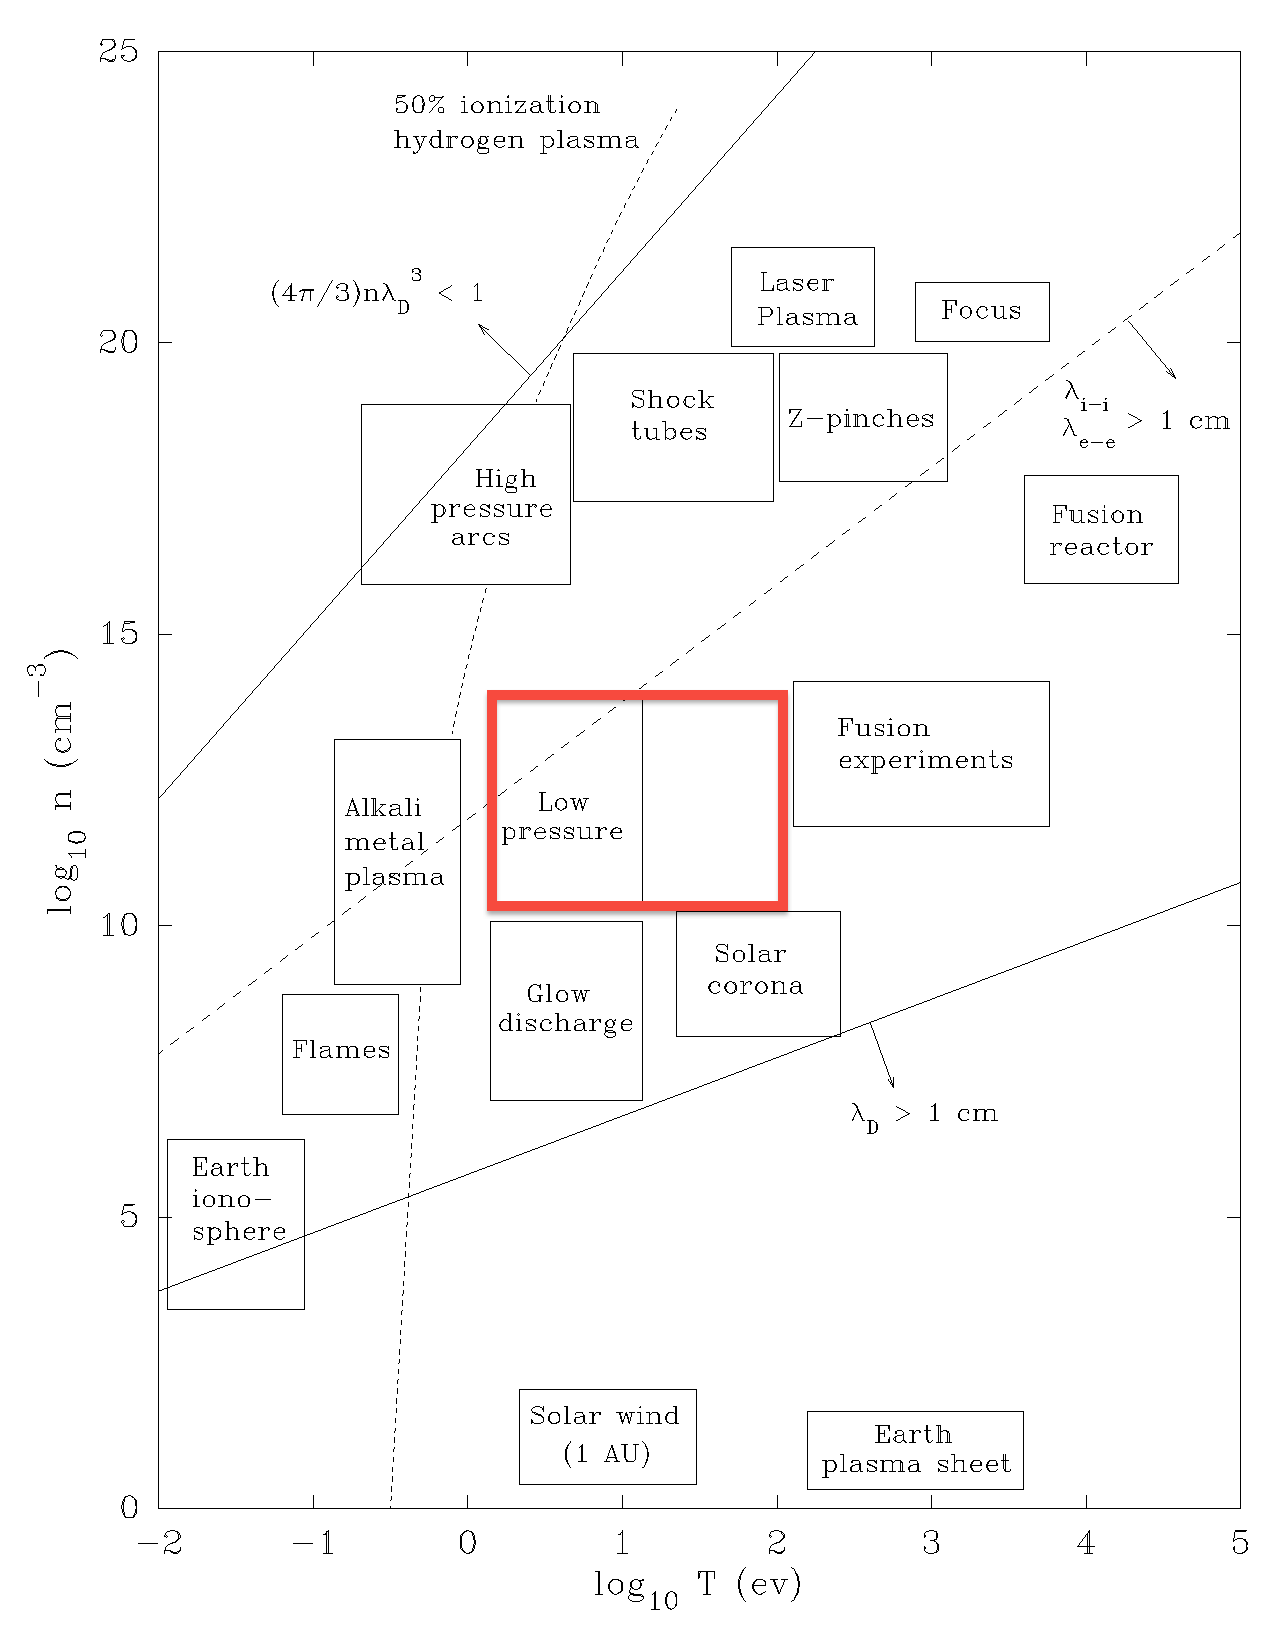
\includegraphics{./chapters/theory/figures/regimes.pdf}
  \caption{Illustration of the various regimes of plasma in terms of
    electron temperature and density with the \acs{rpnd} regime highlighted,
    adapted from \cite{Huba2011}.}
  \label{fig:regimes}
\end{figure}
shows several categories of plasma, plotted as a function of their electron
density and temperature. As can be seen in this example, the electron densities
span seven decades, and the densities cover in excess of 20. This broad range of
conditions presents a particularly challenging problem for both simulations and
experimental measurements. Also highlighted in the figure is the range spanned
by the \acs{rpnd}.

\section{Discharge Initiation}
The Boltzmann equation is a continuous, statistical description of a plasma. By
comparison, the initial breakdown of a plasma is a highly discontinuous process
marked by its stochasticity. The initiation of a discharge is typically the
result of electron avalanches which occur randomly throughout a volume of gas
\cite{Druyvesteyn1940}. Often, the seed electrons for a plasma are the products
of ionizing cosmic rays. At sea level this results in a few electrons per
cubic-centimeter. As a result, it is necessary to consider the initiation of a
discharge separately from a pre-existing plasma.

\subsection{Townsend Mechanism}

Classically, plasmas are created by two different mechanisms, the applicability
of which depends on primarily on the strength of the electric field relative to
the neutral gas density, a value called the reduced electric field
\cite{Huxley1966}. At lower reduced fields, the Townsend mechanism is
responsible for the formation of a plasma. Consider two electrodes separated by
a gap filled with some gas. An electron starting near the cathode will drift
toward the anode. For a large enough electric field, the electron will gain
sufficient kinetic energy to ionize a neutral atom, producing a second electron.
The two electrons are now accelerated by the field, instigating further
ionization of the background gas. The population of electrons quickly grows,
thus the process is referred to as an electron avalanche. Eventually, the
avalanche electrons are collected at the anode.

In their wake are ions which slowly drift toward the cathode. As the ions impact
the surface of the cathode, they occasionally cause a secondary electron to be
emitted. This secondary electron initiates a new avalanche and helps to sustain
the discharge. A steady state electric discharge occurs when the current of the
ion collection at the cathode matches the current of the electron collection at
the anode. The time scale of the Townsend discharge is usually determined by the
positive ions, as their large mass results in slow drift velocities. For an
electric field of 50 V/cm at 200 mTorr, the drift velocity of a helium ion in
helium is about $7\times10^4$ cm/s \cite{Hornbeck1951}. For a gap of 10 cm, this
gives a drift time on the order of $10{-4}$ s.

The Townsend mechanism is characterized by two parameters: $\alpha$ and
$\gamma$, the first and second Townsend coefficients. $\alpha$ is the number of
ionization events that occur per unit length, often expressed as a function of
the reduced field \cite{Druyvesteyn1940}. The second Townsend coefficient is the
probability that an ion impinging on the cathode produces a secondary electron.
The values for $\gamma$ can vary widely and depends on the type of ion, its
energy, the cathode material, contamination of the surface, and many other
factors. That said, typical values are around 0.01-0.1 \cite{Lieberman2005}.

\subsection{Streamer Mechanism}

In contrast, the streamer discharge which occurs for larger values of the
reduced field does not depend on secondary emission. Additionally, streamer
discharges can develop in time periods as short as 1 ns, much less than the time
required for Townsend breakdown. In order to describe the streamer mechanism,
again consider an electron between two electrodes, as seen in (a) of
figure~\ref{fig:streamer}.
\begin{figure}
  \centering
  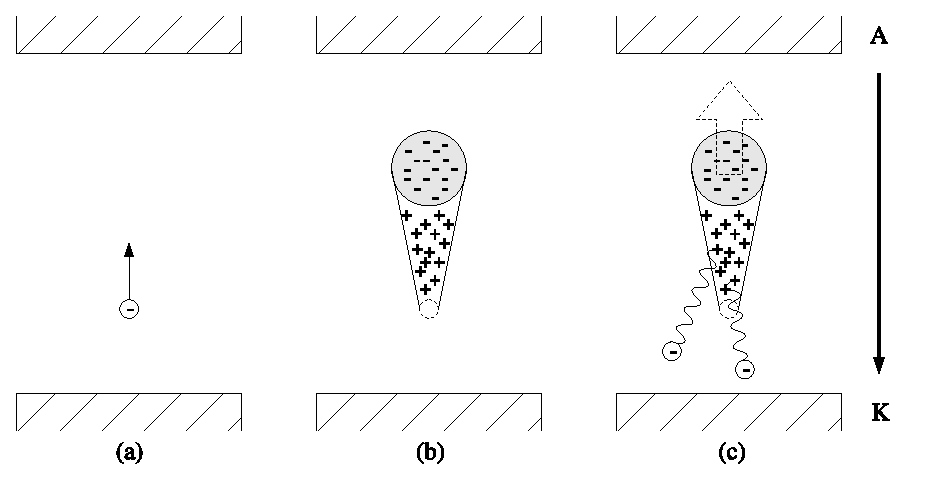
\includegraphics{./chapters/theory/figures/streamer.eps}
  \caption{An illustration of the development of a single streamer. (a)
    A seed electron is accelerated by the applied electric field. (b) The
    initial electron develops into an avalanche which leaves a large region
    of positive space charge, slowing further advance. (c) The streamer
    propagates toward the cathode via photoionization and the anode via
    nonlocal electrons and photoionization. Adapted from \cite{Levatter1980} and
    \cite{Kunhardt1980}.}
  \label{fig:streamer}
\end{figure}
As with the Townsend discharge, this electron initiates an avalanche which moves
toward the anode. As the electrons travel toward the anode, they randomly
collide and diffuse, leaving behind a cone of ions, as seen in part (b).
However, the higher reduced field drastically increases $\alpha$. This causes
the space charge of the avalanche to create an electric field comparable to the
one that is applied, slowing the propagation of the avalanche.

At this point the avalanche can be considered a streamer as it begins to
increase its extent by several additional processes. The large internal fields
of the avalanche can accelerate individual electrons and ``inject'' them in the
direction of the anode \cite{Kunhardt1980}. In addition, as the excited atoms in
the wake of the avalanche begin to radiate, they can cause photoionization
throughout the volume. Photoelectrons generated close enough to the negative
head, or positive tail of the streamer will initiate secondary avalanches which
eventually connect to the primary one. While photoelectrons may cause some
additional broadening of the streamer, the injection of electrons toward the
anode is aligned with the direction of the internal field of the avalanche. As a
result, the ionization caused by these electrons do not appreciably increase the
radius of the streamer.

\subsection{Homogeneity Condition}

However, these processes are not critical in the formation of a large-volume
discharge by an \acs{rpnd}. This description of a streamer only considers an
avalanche generated by a single electron. In reality, many can form
simultaneously assuming that there is more than one seed electron in the volume.
With moderate preionization of the volume, the strong fields of the individual
avalanches can begin to overlap\footnote{If the preionization of the volume is
too large, it can effectively short out the electric field.}. This smoothes out
the field gradients which would otherwise radially constrict the streamers.
Instead, ionization progresses homogeneously throughout the volume.

In order to determine the necessary preionization density, we refer to the work
done by Levatter and Lin on gas laser discharges \cite{Levatter1980}. First, the
electron drift velocity in an applied field can be expressed as the product of
the field and the electron mobility $\mu$. The electron mobility multiplied by
the electric field is the steady-state drift velocity for an electron in that
field and represents the balance between the frictional force of the neutral gas
collisions and the electric field. Consequently, the mean velocity of electrons
drifting in a time-varying field $E(t)$ can be expressed as
\begin{equation}
  u(t) = \mu(E) E(t).
\end{equation}

The length of the avalanche can be written as a time-integrated function of the
electron drift velocity,
\begin{equation}
  \xi = \int_{t_0}^t u(t) dt.
  \label{eq:s_xi}
\end{equation}
Here, $t_0$ is the time at which $E(t)$ becomes high enough that the first
Townsend coefficient, $\alpha$, exceeds 0. Because no electron multiplication
occurs while $\alpha < 0$, this effectively represents the beginning of the
avalanche.

The electric field in the head of the avalanche depends on its radius, which is
dependent on the diffusion of the electrons as they cross the gap. This is
governed by the free diffusion coefficient, $D$. For a fixed diffusion constant,
the final avalanche radius would simply be $R = \sqrt{2D\Delta t}$, where
$\Delta t$ is the time after breakdown. As the diffusion coefficient typically
varies with the applied electric field, the final avalanche radius will be
assumed to be equal to $R = \sqrt{2\bar{D}\Delta t}$, where $\bar{D}$ is the
time-averaged diffusion coefficient.

Levatter and Lin assume that the avalanche slows when the peak field of the
avalanche is equal to the applied field. Assuming that the electrons diffuse
equally in all directions, the electric field of the avalanche head can be
expressed as
\begin{eqnarray}
  E_a(r) = \frac{eN_e}{4\pi\epsilon_0R^2} F(r/R), \qquad \mathrm{where} \\
  F(r/R) = \frac{1}{R^2}\left[\mathrm{erf}(r/R)-\frac{2}{\pi^{1/2}}
           (r/R)\exp(-r^2/R^2)\right] ,
\end{eqnarray}
where $r$ is the radius with respect to the center of the avalanche, $N_e$ is
the number of electrons in the avalanche, $\mathrm{erf}$ is the error function.
$F$ is a dimenionless function which has a peak value of $0.428$. Provided
$\alpha$ as a function of reduced field, the number of electrons in the
avalanche is equal to
\begin{equation}
  N_e = \int_0^\xi \alpha(\xi')d\xi'.
  \label{eq:s_pop}
\end{equation}

Here, Levatter and Lin make a number of assumptions in order to develop an
analytic and dimensionless solution for $E_{a,\mathrm{max}}(t) = E(t)$. However,
it is possible to numerically integrate equations~\ref{eq:s_xi},~\ref{eq:s_rad},
and~\ref{eq:s_pop} to determine the time required for the avalanche to slow.
This should provide a more accurate, but less general result. Assuming a
linearly increasing electric field, figure~\ref{fig:avalanche_lengths}
\begin{figure}
  \centering
  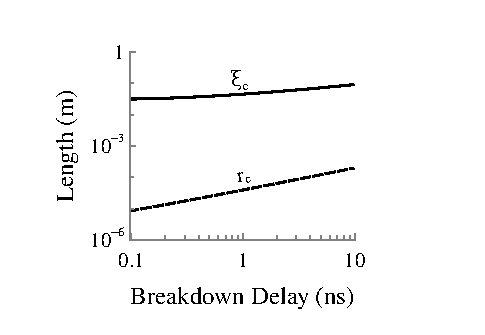
\includegraphics{./chapters/theory/figures/avalanche_lengths.eps}
  \caption{Numerical calculations of the avalanche length and avalanche radius for
    in helium at a pressure of 4.0 Torr as a function of the slope of the electric
    field, $dE/dt$.}
  \label{fig:avalanche_lengths}
\end{figure}
shows the results of such calculations for an avalanche in 4.0 Torr of helium,
as a function of various breakdown delays. The breakdown delay is defined as the
time it takes for $\alpha > 0$. The mobilities, diffusion coefficients, and
Townsend coefficients were interpolated from solutions of the Boltzmann equation
provided by the BOLSIG+ code with Phelps' cross sections \cite{Phelps2002}. For
this range of breakdown delays, the avalanche was able to develop up to nearly
10 cm in length before it slowed. The times required for the avalanche to slow
ranged from around 23 ns for the shortest breakdown delay, and 389 ns for the
longest.

From this, a criteria for homogeneous breakdown of the gas can be developed. In
order for the field gradients to be smoothed out, the individual avalanche heads
should roughly overlap by the time they have slowed. Assuming that all seed
electrons in the volume initiate avalanches, this can be approximated as
$n_{e,c} > r_c^{-3}$, where $n_{e,c}$ is the critical electron density, and
$r_c$ is the avalanche radius when it has slowed. As seen in
figure~\ref{fig:avalanche_densities},
\begin{figure}
  \centering
  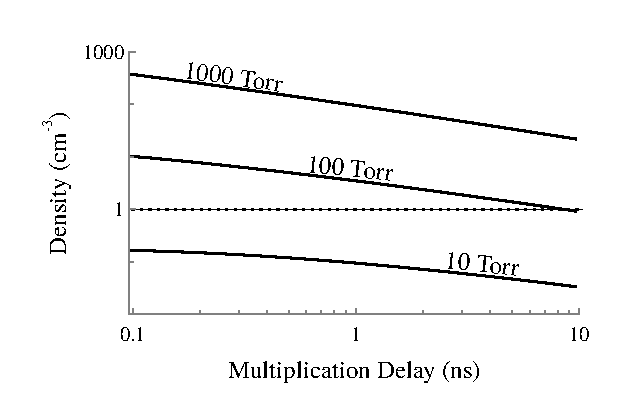
\includegraphics{./chapters/theory/figures/avalanche_densities.eps}
  \caption{Minimum preionization densities required at a variety of pressures
    and breakdown delays. The dotted line indicates the background ionization
    level as a results of cosmic radiation.}
  \label{fig:avalanche_densities}
\end{figure}
the required preionization density depends on both the breakdown delay and the
operating pressure. Generally, the preionization density increases with pressure
and decreases with breakdown delay. The dotted line in the figure indicates the
anticipated background electron density from cosmic radiation. This suggests
that, for the breakdown delays in question, the discharge will almost always be
homogeneous at pressures below 100 Torr. While the plot suggests that large
values of $dE/dt$ might guarantee homogeneous breakdown at near-atmospheric
pressure, the increasing likelihood of ionization instabilities \cite{Johns1972}
will preclude homogeneous discharge development.

\section{Atomic Spectroscopy \& Notation}

As described, much of the experimental work presented will concern the use of
spectroscopic techniques. Careful measurements of the light emitted from excited
atomic states can yield electron densities and temperatures, excited state
densities and temperatures, electric fields, and magnetic fields
\cite{Griem2005}. The topic of spectroscopy is extensive and it is neither
necessary nor desirable to cover it in full. Instead we will only consider what
is necessary to understand the emissions from a singly-excited, multi-electron
atom.

An atom is composed of a small, positively charged nucleus, orbited by
negatively charged electrons. The actual position of any single electron is
probabilistic and described by a wavefunction--solutions of the Schr\"{o}dinger
equation for the atom in question. Each wavefunction is associated with a number
of eigenvalues which quantize aspects of the state of bound electrons. In simple
atoms, four such quantum numbers are of interest \cite{Drake2006},
\begin{itemize}
  \item $n=1,2,\ldots$: the principal quantum number,
  \item $l=0,1,\ldots,n-1$: the orbital angular momentum number,
  \item $m_l =-l,\ldots,l$: the projection of $l$, and
  \item $m_s=\pm1/2$: the projection of the spin quantum number.
\end{itemize}
The quantum numbers are hierarchical such that each $n$, or shell, possesses a
series of subshells, $l$, while each subshell possesses a number of individual
orbital, $m_l$, and each orbital possess one of two spins. As a result of the
Pauli exclusion principle, the wavefunction of each electron around an atom is
described by a \emph{unique} set of quantum numbers. This means, that any
particular subshell can only contain $2(2l+1)$ electrons. The subshells are
often referred to using the nomenclature $0,1,2,3,\ldots = s,p,d,f,\ldots$.

As a result of their separation from the nucleus, the electrons in an atom
possess some degree of potential energy. As the $n$ and $l$ of an electron
increase, so does its potential energy. In the absence of electric and magnetic
fields, $m_l$ and $s$ do not affect the potential energy of an electron. As an
example, an electron in the 1s ($n=1$ and $l=0$) subshell has the lowest
possible potential energy.

Absent from external influences, the individual states are populated with
electrons so as to minimize the total potential energy of the system. This
natural arrangement is referred to as the ground state configuration. Often, but
not always, the subshells are filled sequentially and in order from lowest to
highest $l$ \cite{Drake2006}. Provided some input energy in the form of a
collision or a photon, one or more of the electrons surrounding the atom may
transition to another state, increasing the potential energy of the system. In
low-temperature plasmas it usually one of the electrons from the outermost or
partially filled subshell to be excited.

The potential energies of the electron configurations for multi-electron atoms
are determined by the collective effects of all the surrounding electrons.

It is the collective effects of all electrons surrounding an atom which
determine its potential energy. This results in a single set of total angular
momenta which can be used to describe the atom. In lighter atoms
\cite{Drake2006}, the contributions of the individual electrons are combined
assuming a condition called L-S coupling. Under this assumption, the total
angular momentum of the atom can written as $\vec{L} = \sum\vec{l}_i$, where $i$
is each electron in a partially filled subshell (filled subshells sum to zero).
Likewise, the total spin can be written as $\vec{S} = \sum\vec{s}_i$. These can
be combined to form the total angular momentum of the atom, $\vec{J} = \vec{L} +
\vec{S}$. Finally, the each atom is said to have an even or odd parity, defined
as $(-1)^{\sum\bm{l}_i}$, where $-1$ is odd, and $1$ is even.

These quantities can be used to write a ``term symbol'' for the atom, of the
form $^{2S+1}L_J^p$, where $p$ is `o' if the parity is odd, and omitted if it's
even. The term symbol can be augmented by prepending additional terms which
address the subshells in which electrons can be found. This is typically written
as $nl^N$, where $N$ is the number of electrons in a given subshell (ommitted if
$N=1$). For example, 1s2s$^3$S$_{1}$, describes the triplet helium metastable
state. In this case, there is a single electron in the 1s subshell and a second
atom in the 2s subshell. The configuration has a total orbital angular momentum
of 0 (denoted by the `S'), an even parity (denoted by the absence of a
superscript `o'), a total spin of $1$ (the superscript $3$ is equal to $2S+1$),
and a total angular moment of 1.

Excited atomic states usually have finite lifetimes. Normally, electrons will
undergo transitions to lower the potential energy of the system. This can also
occur spontaneously, through the emission of a photon, or through a superelastic
collision with another particle. In the case of spontaneous transitions, only
certain states can transition to others, as defined by a series of selection
rules \cite{Drake2006}:
\begin{itemize}
  \item $\Delta S = 0$
  \item $\Delta L = \pm1$ or 0
  \item $\Delta J = \pm1$ or 0
  \item $L=0$ cannot transition to $L=0$
  \item $j=0$ cannot transition to $J=0$
\end{itemize}
These rules are determined from a lower order approximation, and thus are not
strict. As a result, forbidden transitions can occur, however these generally
take place at much lower rates.

Figure~\ref{fig:grotrian}
\begin{figure}
  \centering
  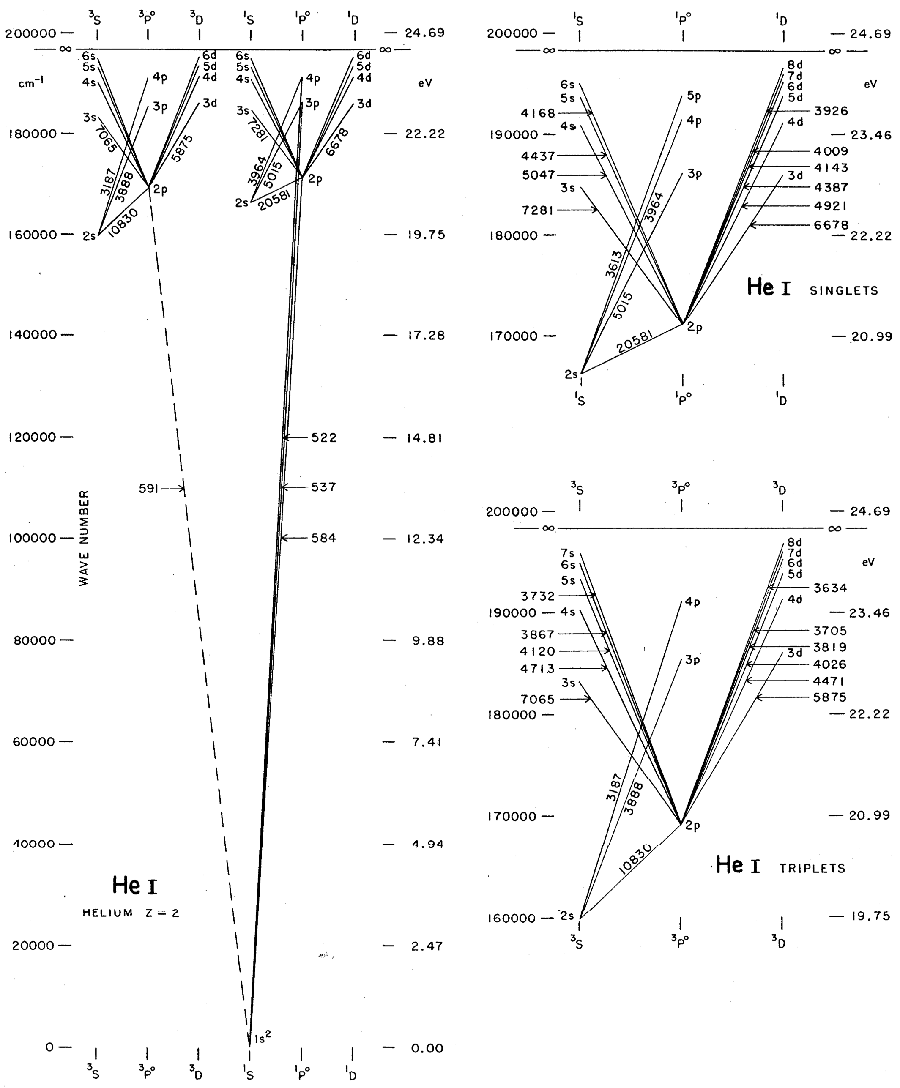
\includegraphics{./chapters/theory/figures/grotrian.pdf}
  \caption{A partial Grotrian diagram of neutral helium, from \cite{Moore1968}.}
  \label{fig:grotrian}
\end{figure}
is a Grotrian diagram of the energy levels in neutral helium and the allowed
transitions. In this case, the atomic states are separated into the singlet
($S=0$) and triplet ($S = 1$) manifolds. The singlet manifold is composed of
excited states where the electron spins are anti-parallel, and the triplet
manifold represents excited states where the electron spins are parallel. As
indicated by the first selection rule, transitions between these two manifolds
is forbidden, thus each is something of a self-contained system
\cite{Herzberg1944}.

Also observable in the diagram are two ``metastable'' states. These are the 2s
states at the bottom of the singlet and triplet manifolds. An electron in either
state cannot spontaneously transition to a lower energy state. As a result, an
electron in either state can be extremely long-lived. In addition, they are also
the lowest-lying excited states of helium. For these reasons, helium plasmas
tend to have high densities of metastable atoms. This makes them a good
candidate for spectroscopic study as will be seen in
chapter~\ref{chp:metastables}.

\subsection{Spectral Lineshapes}

Electrons which transition to lower energy states emit photons which can be
detected. Conversely, if an atom is exposed to a photon with an energy matching
a transition, the atom may absorb the photon. Both processes are useful in
determining the prevalence and dynamics of the excited states. This, in turn,
can be used to infer various plasma properties.

Conservation of energy requires that the energy of the absorbed or emitted
photon match the energy difference between the two states. However, the finite
lifetime of excited atomic states implies, via the time-energy formulation of
the uncertainty principle, some uncertainty in the actual energy difference
between the states. As a result, the emitted photon will possess an energy
selected from a distribution of energies.

This distribution is referred to as the spectral lineshape. The narrowest
permissible lineshape, or natural lineshape, of an atomic transition can be
shown \cite{Siegman1986} to be a Lorentzian of the form,
\begin{equation}
  g(\omega) = -\frac{1}{4\pi^2}\frac{A\lambda^3}{\dwa}
  \frac{1}{1 + \left[2(\omega-\omega_a)/\dwa\right]^2},
  \label{eq:lorentzian}
\end{equation}
where $\omega$ is the photon frequency, $A$ is the Einstein coefficient for the
transition, $\lambda$ is the wavelength of the transition, $\omega_a$ is central
frequency of the transition, and $\dwa$ the full-width half maximum (\acs{fwhm})
of the transition. In the ideal case, where the atoms motionless and unaffected
by external perturbations, $\dwa = A$ \cite{Siegman1986}. This is known as the
natural linewidth.

Other processes can act to broaden or alter the spectral lineshape
\cite{Kunze2009}. For example, inter-atomic collisions can reduce the lifetimes
of excited states. This results in additional broadening of the line, though it
retains its Loretnzian nature. As the frequency of inter-atomic collisions
increases linearly with pressure, this phenomena is referred to as pressure
broadening. It can be included in equation~\ref{eq:lorentzian} by using $\dwa =
A + BP$, where $B$ is a measured or calculated broadening coefficient, and $P$
is the pressure \cite{Siegman1986}.

Atomic motion can also play a role in the spectral lineshape. If an atom is
moving toward or away an observer as it emits a photon, the emitted photon will
be blue or red shifted. Likewise, if the atom is moving toward or away an
incident photon, the energy of that photon will be shifted \cite{Siegman1986}.
If this effect is averaged over the random motion of atoms in a gas, the result
is an additional broadening of the lineshape, called Doppler broadening. Unlike
pressure broadening, Doppler broadening introduces a Gaussian component to the
lineshape such that,
\begin{multline}
  g(\omega) = \sqrt{\frac{2\ln{2}}{\pi^3}}\frac{\dwa}{\dwd}
  \int_{-\infty}^\infty
  \frac{1}{[(\omega - \omega_a) - \omega']^2 + 4\dwa^2} \\
  \times \exp\left[4\ln{2}\left(\frac{\omega'}{\dwd}\right)^2\right]d\omega'.
  \label{eq:voigt}
\end{multline}
Here, $\dwd = \omega_a\sqrt{\frac{8k_\mathrm{B}T_\mathrm{g}\ln{2}} {Mc^2}}$, is
the width of the Doppler broadening, where $T_g$ is the gas temperature, $M$ is
the particle mass, and $c$ is the speed of light. This form of the spectral
lineshape is known as the Voigt profile, and it must be numerically integrated.
In the case that $\dwd >> \dwa$, equation~\ref{eq:voigt} can be simplified to a
standard Gaussian distribution,
\begin{equation}
  g(\omega) = \sqrt{\frac{4\log{2}}{\pi\dwd^2}}
  \exp\left[-(4\log{2})\left(\frac{\omega-\omega_a}{\dwd}\right)^2\right].
\end{equation}

The effect of the various broadening mechanisms is most apparent in the wings of
the lineshape, far from the peak. Figure~\ref{fig:lineshapes}
\begin{figure}
  \centering
  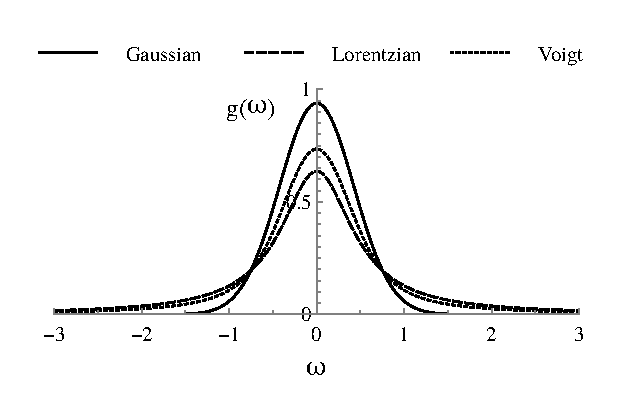
\includegraphics{./chapters/theory/figures/lineshapes.eps}
  \caption{A comparison of the three primary spectral lineshapes, each with the
  same full width.}
  \label{fig:lineshapes}
\end{figure}
illustrates the three major lineshapes with equivalent full widths. The Voigt
profile is composed of equally broad Lorentzian and Gaussian distributions. As
can be seen, the wings of the Gaussian distribution fall off very quickly. In
comparison, the Lorentzian component is observable well out to the edges of the
figure. 

The spectral lineshape can be altered by a number of other processes. Electric
fields can influence the emissions via the Stark effect, while magnetic fields
can split up degenerate states via the Zeeman effect. The fields of electrons
and nearby molecules can also alter the lineshape of a transition. While not
used in this study, such effects can be used as effective diagnostic tools in
the measurement of field strengths, and charged particle densities in plasmas.

\subsection{Absorption}

As has been mentioned, a photon which closely matches the energy between two
states can be absorbed by an atom. This property forms the basis for absorption
spectroscopy where light with a known spectrum is used to illuminate a sample.
The spectrum of the light that passes through the sample is measured and used to
infer properties of the sample. In contrast to the emission processes occur
spontaneously with a characteristic lifetime, often 10s of nanoseconds or more,
absorption is almost instantaneous. This makes absorption-based spectroscopic
methods desirable for fast phenomena, such as the \acs{rpnd}
\cite{Demtroder2008}.

The cross section for a single atom to interact with a photon can be shown
\cite{Siegman1986} to be,
\begin{equation}
  \sigma(\omega) = A \frac{\lambda^2}{8\pi}\frac{g_1}{g_2}g(\omega).
  \label{eq:absorb}
\end{equation}
where $g_1$ and $g_2$ are the number of degenerate configuration for the lower
state and upper state respectively. $g(\omega)$ is the appropriate spectral
lineshape, determined from the operating conditions.

It is important to recognize that absorption spectroscopy can also perturb the
system it is measuring. Suppose two consecutive photons were incident on the
atom. If the first was absorbed, the likelihood that the second photon would be
absorbed is zero. The cross section for absorption has not changed, there are
simply no atoms available for the second photon to interact with. Therefore, if
a photon field is incident on a volume of atoms susceptible to absorption, the
degree to which the field is absorbed will depend on its intensity. The more
intense the photon field is, the more it reduces the number of atoms available
to interact with.

Eventually, this effect is balanced by a process called stimulated emission. In
this process, an atom is already in an excited state with one or more lower
states. If an photon is incident on the atom and matches the energy difference
between its current state and a lower one, the photon may induce a transition to
the lower state. This results in the emission of a second photon with the same
energy and phase as the first. The cross section for stimulated emission is
identical to that for photon absorption.

This feedback process where the absorption and emission processes balance with
each other is known as saturation. The saturation of a volume of gas is a
continuous process, and depends on the atomic states in question and areal
density of the incident photons, or intensity. From a practical standpoint,
absorption measurements require that the interrogating photon field remain below
a threshold value. This saturation intensity can be shown \cite{Siegman1986} to
be,
\begin{equation}
  I_s = \frac{2\sqrt{2}h\nu_0A}{\lambda^2},
\end{equation}
where $h$ is Planck's constant, and $\nu_0$ is the nominal frequency of the
transition \cite{Siegman1986}.

In this report, absorption and spontaneous emission diagnostics provide the
experimental basis on which the \acs{rpnd} analyzed. Both are direct measures of
the excited states that exist within a \acs{rpnd}. However, neither provides any
direct measurement of the quantity or energies of the electrons. In the
\acs{rpnd}, as with all plasmas, the electrons play a fundamental role in how
the discharge behaves and develops. At the most basic level, it is the electrons
which are accelerated by the electric field and collide with the gas atoms to
produce the aforementioned excited states. Consequently, it should be possible
for a sufficiently detailed model to use measurements of the excited states in
order to infer the properties of the electrons, as will be seen in
chapter~\ref{chp:modeling}.


  \chapter{Experiment}\label{chp:exp}
    \section{Discharge Apparatus}

The design of the discharge apparatus was similar to the coaxial geometry used
by Vasilyak and others \cite{Vasilyak1994}. This configuration has the benefit
of minimizing the inductance of the system, which should aid in the propagation
of the pulse through the system. Figure~\ref{fig:appschem}
\begin{figure}
  \centering
  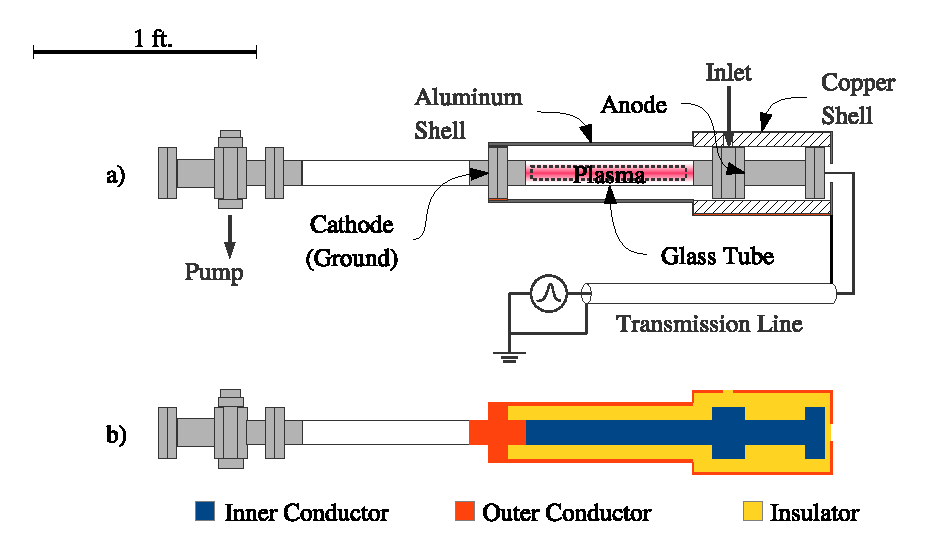
\includegraphics{./chapters/experiment/figures/appschem.eps}
  \caption{A scaled illustration of the discharge apparatus used in the
  \acs{rpnd} experiment.}
  \label{fig:appschem}
\end{figure}
is a to-scale illustration of the discharge apparatus.

The main portion of the discharge was provided by a borosilicate glass tube with
Conflat flanges on either end. The glass portion of the tube had an inner
diameter of 3.3 cm, an outer diameter of 4.0 cm, and a length of 22.9 cm. The
total length of tube, including the glass tube, glass-to-metal transition, and
flanges was 30 cm. The flanges served as the electrodes for the plasma. Seen
here, the anode is located on the right, and the cathode/ground is located on
the left.

The cathode was connected to a second glass tube with the same dimensions as the
first. This tube led to the pumping apparatus and served to electrically isolate
it from the rest of the system. The cathode was also connected to ground through
a cylindrical ground shell\footnote{While all of the outer conductors of the
system are nominally at ground, it is believed that they would float to finite
voltages with each pulse. This is a product of the nonideal impedance to ground
and the high frequencies associated with the fast pulse.} which ran along the
outside of the discharge tube. The ground shell was held in place against the
cathode with a copper shim and Delrin shaft collar.

Two slots were milled into the ground shell on opposite sides. The slots were
3.8 cm by 30 cm and served to provide optical access to the discharge tube. The
side of the ground shell opposite the cathode terminated at a copper sheet, 10
cm square. The copper sheet was perpendicular to the axis of the discharge tube
and had a 5 cm hole for discharge tube to pass through. The ground shell was
connected to the copper sheet with conductive copper tape.

The copper sheet was secured to a Teflon tube, approximately 20 cm in length
with an inner diameter of about 7.5 cm and an outer diameter of 10 cm. The
Teflon tube provided electrical isolation for the anode from structures
supporting it. Surrounding the Teflon tube was a second ground shell composed of
copper. This was connected to the first ground shell by a braided copper strap.
The other end of the second ground shell ended in a similar square copper sheet,
10 cm on each side. This sheet was secured to the Teflon tube by nylon screws
and seated against the ground shell for electrical contact.

The copper sheet also featured a HN bulkhead adapter for connection to the
transmission line. The inner conductor of the bulkhead adapter was connected by
a straight run of 5 cm of silicone-coated wire to a Conflat window angled at
45$^\cdot$. The window was connected to a Conflat nipple, which in turn was
connected to a double-sided flange used as the gas inlet (access was provided by
a 2.54 cm diameter hole drilled into the surrounding Teflon tube). The other
side of the double-sided flange was connected to the anode of the discharge
tube.

The voltage pulse was provided by a \acs{fid} pulser, supplied by \textsc{anvs},
Inc. (model \smaller{PT510NM}). The amplitude of the pulse was fixed at 6.4 kV
with a repetition rate of 1.0 kHz. Each pulse had a fixed width of 25 ns, with a
10\%-90\% rise time of approximately 4 ns and a roughly Gaussian shape. It is
likely that the low conductivity of the gas preceding each pulse resulted in a
doubling of the pulse potential as it reflected from the electrode. A
\textsc{srs} \smaller{DG645} delay generator was used as the master clock in all
experiments and was used to trigger the pulser. A 13.7 m transmission line was
used in order to isolate reflections traveling back and forth between the pulser
and anode. The cable used was RG213, and HN connectors were used to prevent
breakdown between the center conductor and ground.

The gas inlet connection was made through the double-sided flange via a 1/8"
\textsc{npt} hole. A 1/4" polyethylene tube was attached to the \textsc{npt}
connection via a \textsc{npt} to 1/4" Swagelok adapater. The tube was then
connected by Swagelok to a source of ultra-high purity (99.999\%) helium.
Throughout the experiment, the helium flow rate was fixed at 25.0 sccm with a
digital flow controller, regardless of the operating pressure.

The discharge apparatus was pumped down by a oil-based roughing pump with an
upstream zeolite trap. In each case, the system was evacuated by the roughing
pump to the base pressure, approximately 15 mTorr, via a large-diameter tube.
Based on this, the level of background impurities was estimated to be 80 ppm.
This pump path was the closed off, and additional pumping was performed via two
needle valve bypasses. The needle valves were used to adjust the pump rate in
order to obtain the desired system pressure, monitored by two capacitance
manometers with ranges of 10 and 100 Torr.

The assembled discharge apparatus can be seen in figure~\ref{fig:appphoto}.
\begin{figure}
  \centering
  \setlength\fboxsep{0pt}
  \setlength\fboxrule{1.0pt}
  \fbox{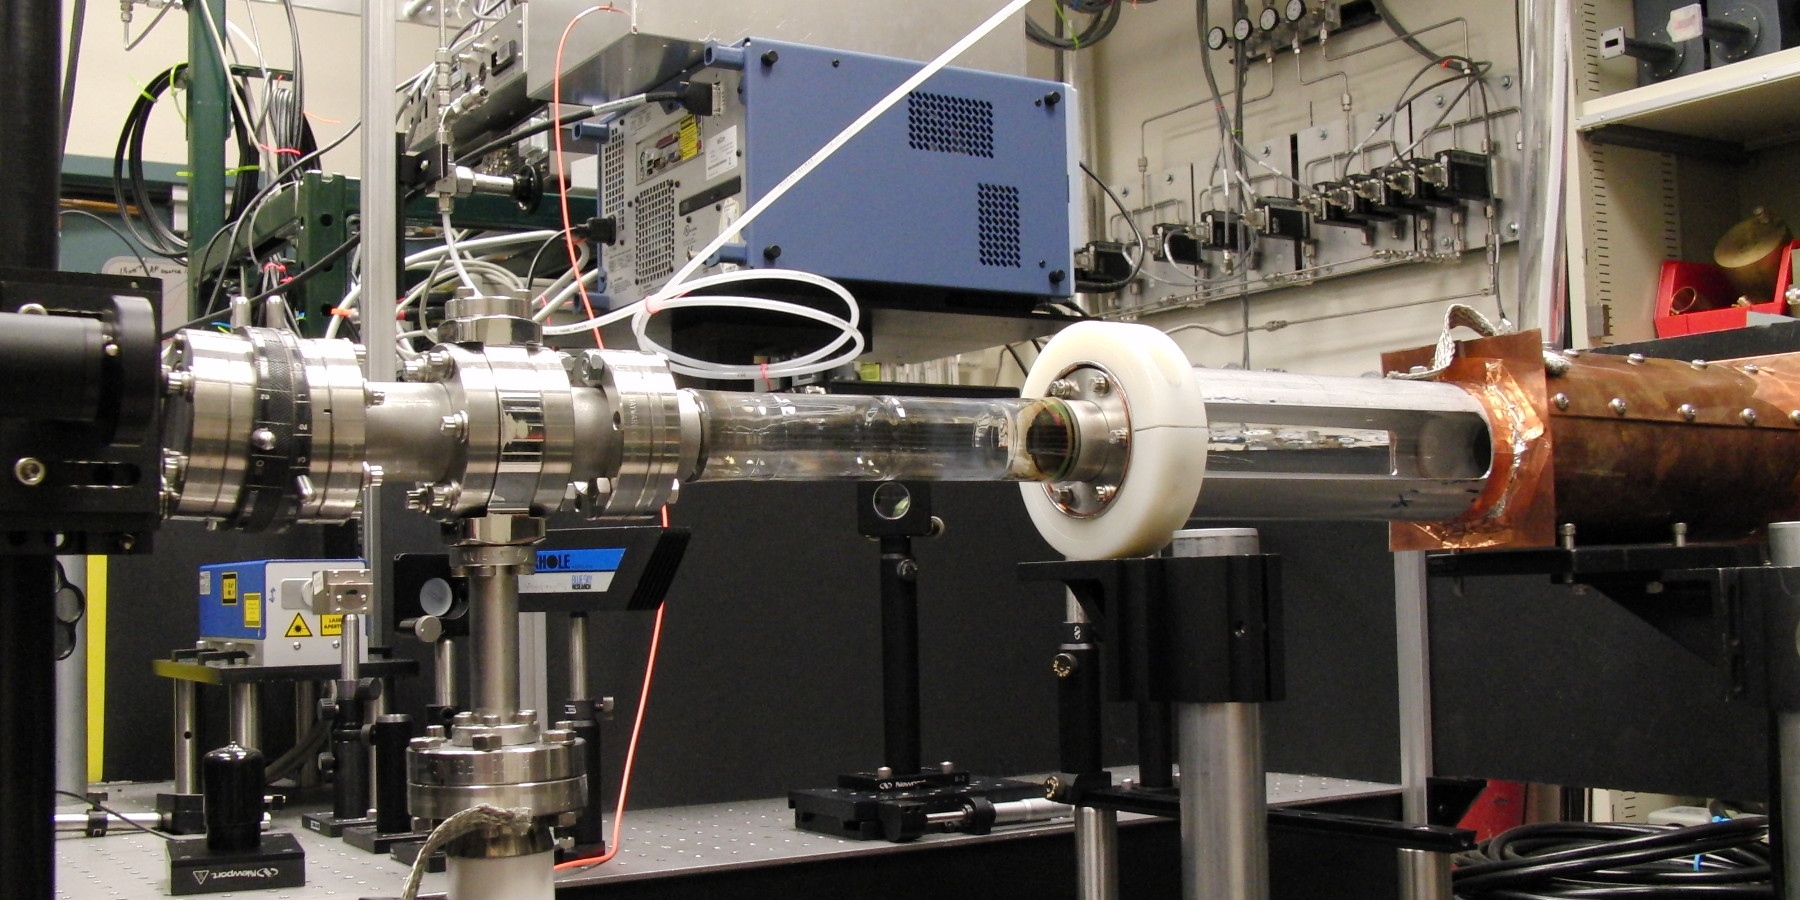
\includegraphics{./chapters/experiment/figures/appphoto.jpg}}
  \caption{Photograph of the discharge apparatus.}
  \label{fig:appphoto}
\end{figure}
The apparatus was supported on an optical breadboard 2.54 cm diameter posts and
angle brackets. Attached to one of the angle brackets was a small optical
breadboard with four bolts which served as physical references for aligning and
positioning the apparatus.

All electrical measurements were made with a LeCroy \smaller{6100A} WaveRunner
oscilloscope which had a bandwidth of 1.0 GHz. Electrical connections to the
oscilloscope were made with the shortest practical lengths of \smaller{RG 50/U}
coaxial cable and terminated at 50 $\Omega$ unless otherwise noted. The voltage
of the pulser was monitored from an internal $1:1000$ divider, and the current
was via a current shunt located in a break of the outer conductor of the
transmission line. The current shunt was composed of 9, low inductance, $1.0
\Omega$ resistors connected in parallel. Figure~\ref{fig:bcs}
\begin{figure}
  \centering
  \setlength\fboxsep{0pt}
  \setlength\fboxrule{1.0pt}
  \fbox{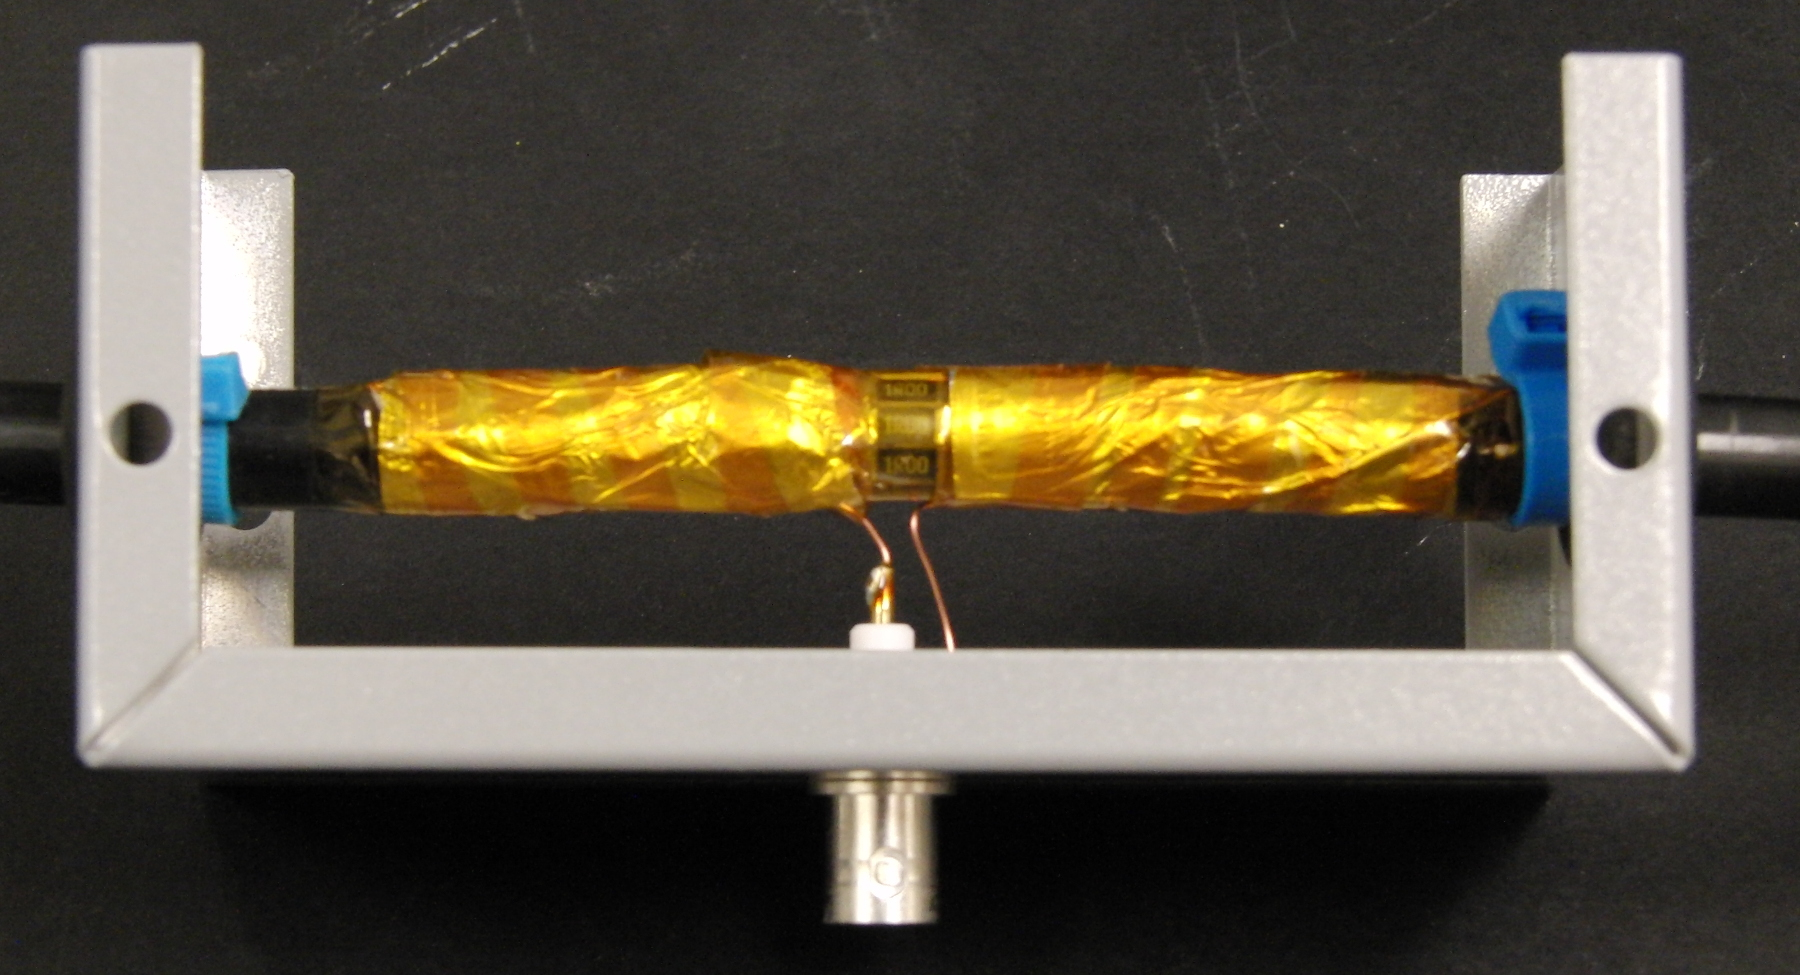
\includegraphics{./chapters/experiment/figures/bcs.jpg}}
  \caption{Photograph of the back-current shunt used to measure the current
  characteristics of the \acs{rpnd}.}
  \label{fig:bcs}
\end{figure}

Data were retrieved from the oscilloscope with a desktop computer via a
\textsc{gpib} connection. A LabView interface was used to interface with the
oscilloscope and additional instruments. Analog inputs and outputs (such as
laser control and pressure sensing) were handled by a \textsc{srs}
\smaller{sr850 dsp} lock-in amplifier which performed as an \emph{ad hoc} data
acquisition system.

\section{Operating Procedure \& Conditions}

At the beginning of each day of operation, the system was first pumped down to
base pressure. After this, the primary pump path was closed in favor of the
needle valve bypasses. The helium flow was then initiated at 25.0 sccm. Then,
the system pressure was adjusted to 3.0 Torr.

Once the pressure reached equilibrium, the pulser was turned on. The plasma was
allowed to run at this condition for one hour in order to remove built up
contamination on the walls and electrodes. During this time, the pressure of the
system would typically drift downwards by several percent. Afterward, the
pressure would be adjusted to the desired operating condition.

It was frequently necessary to turn off the pulser in between experiments. In
these cases, once the pulser was turned on, the plasma was allowed to run for 15
minutes before any measurements were made. This was necessitated by observable
changes in the emissions and current-voltage characteristics during the first 15
minutes of operation. Additional increases to this warm up time resulted in no
appreciable changes to any of the measured data.

Measurements were made for a range of pressures, including: 0.3, 0.5, 1.0, 2.0
3.0, 4.0, 8.0, and 16.0 Torr. The lower limit was set by the pumping speed of
the roughing pump. Difficulty in obtaining reliable plasma breakdown at
pressures above 16.0 Torr set an upper limit on the pressure range. Experimental
measurements of optical properties were obtained at three axial locations: 7.6,
15.2, and 22.9 cm, relative to the anode. These will frequently be referred to
as upstream, midstream, and downstream locations, respectively.

\section{Initial Observations}

Plasma characteristics could be divided into approximately three cases: low,
intermediate, and high pressure. At the low pressures, 0.3, 0.5, and 1.0 Torr,
it was difficult to initiate a discharge. Frequently, the plasma would have to
be started at more moderate pressures, and then adjusted to the desired
condition. At these conditions, the plasma was dim compared to the ambient room
light and a dull purple. It appeared to be well separated from the walls.
Visually, the diameter of the plasma was estimated to be about 2 cm, however
this increased with pressure. Also occurring at these conditions was a large
amount of electronic noise. Nearby instruments, such as the computer mouse, and
lock-in amplifier, would occasionally malfunction at these conditions.

At moderate pressures, 2.0, 3.0, and 4.0 Torr, the plasma expanded radially to
fill the whole of the discharge volume. Compared to ambient conditions the
plasma was bright with an orange-pink hue. Electrical interference disappeared
at these conditions, and the plasma initiation was relatively easy.
Nevertheless, at the beginning of each day several thousand pulses could be
required before a visible plasma was formed. Interestingly, the plasma extended
well past the cathode/ground and to the pumping section (connected to ground at
a separate point). Presumably, this is a result of the relatively small cathode
area compared to the large anode area. The build up of space charge limits the
current extraction from the intended cathode, subsequently the electrode further
downstream begins to contribute.

For the higher operating pressures, 8.0 and 16.0 Torr, the brightness of the
plasma decreased, though not to the level of the low pressure discharge. In
addition, the plasma remained volume-filling. However, it did not visibly
extended past the cathode. Discharge initiation was difficult at these operating
conditions and, as in the low pressure case, the plasma would have to be started
at more amenable conditions. No electrical interference was noted for this
pressure range.

Cursory examination of the voltage signal revealed a large number of reflections
in the system. These can be seen in figure~\ref{fig:waveform},
\begin{figure}
  \centering
  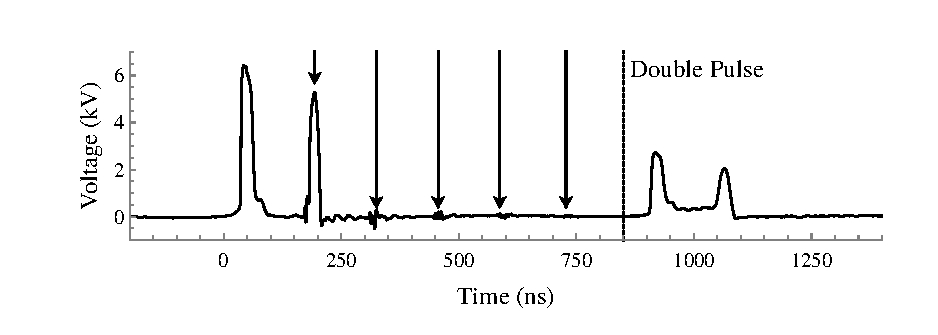
\includegraphics{./chapters/experiment/figures/waveform.eps}
  \caption{Typical voltage waveform of the \acs{rpnd}. Arrows indicate
  reflections back to the pulser. The pulser exhibited a double pulsing
  phenomena, indicated by the dotted line.}
\end{figure}
a typical voltage waveform with overlaid arrows indicating the reflected pulses.
These can be attributed to the impedance discontinuity at the electrode. Also
observable in the waveform is a second pulse and its associated reflection. This
is believed to be a peculiarity of the particular power supply used. The
majority of the presented results, particularly those concerning the fast
dynamics will only consider the initial pulse.

\section{Field Calculations}

The electric field characteristics of the discharge system was analyzed using a
two-dimensional, electrostatic solver, Ansoft Maxwell 9. Figure~\ref{fig:fields}
\begin{figure}
  \centering
  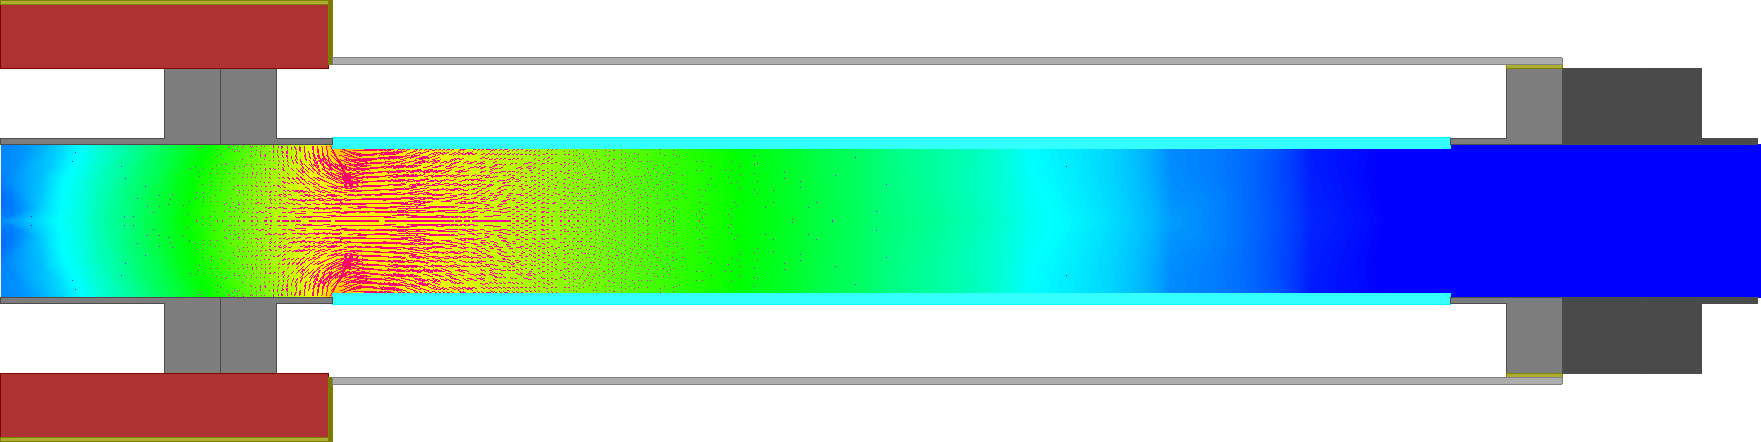
\includegraphics{./chapters/experiment/figures/fields.jpg}
  \caption{Heat map and vector plot of the electric field in the \acs{rpnd}
  discharge apparatus.}
  \label{fig:fields}
\end{figure}
is a logarithmic heat map of the electric field magnitude, with overlaid
electric field vectors (in magenta). The electric field varies significantly
over the length of the discharge apparatus, with a peak near the axial location
of the glass tube followed by a monotonic decline. These characteristics are a
large departure from simple case of two parallel electrodes in which the field
is uniform throughout. This can be attributed to the presence of the external
ground shield. Though this does complicate the field characteristics, the
proximity of the ground results in a much higher electric field than would
otherwise be achievable.

While the off-axis field lines all feature notable radial components,
particularly close to the anode the center line does not.
Figure~\ref{fig:centere}
\begin{figure}
  \centering
  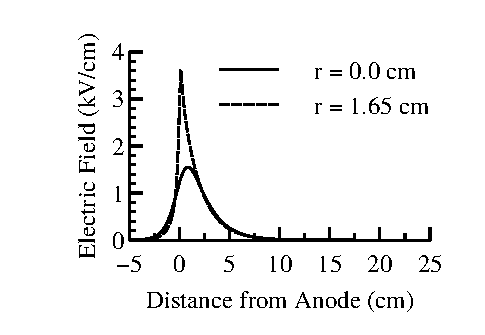
\includegraphics{./chapters/experiment/figures/centere.eps}
  \caption{The magnitude of the electric field along the center and outside of
  the discharge apparatus.}
  \label{fig:centere}
\end{figure}
is a plot of the magnitude of the electric field along the central axis of the
discharge apparatus and the outside, adjacent to the glass tube. The location of
the anode is defined as the location of the glass-to-metal seal.

\section{Energy Coupling}



\section{Absorption Setup}
The \acs{las} setup was based upon the used of a distributed-feedback
laser diode. Temperature and current control of the diode provided
coarse and fine tuning, respectively, for the output frequency. It was
found that it was unnecessary to adjust the temperature for the diode
once the correct transition was found, therefore all tuning was
accomplished using current tuning.

The laser diode was produced by Toptica Photonics (model
\#LD-1083-0070-DFB-1), and had a nominal operating power of 70 mW at a
center wavelength of 1083 nm. The diode was held inside a Toptica DL-100
diode housing which contained an integral thermoelectric cooler and
collimating optics. The operation of the diode was controlled by a
Toptica DC 110 monitor, DCC 110 current control, DTC 110 temperature
control, and SC 110 scan control.

A schematic of the optical layout for the absorption experiment can be
seen in Figure \ref{fig:abslayout}. Immediately after exiting the
housing, the beam was passed through an optical isolator in order to
prevent instabilities from back reflections. Next the beam was
attenuated using a neutral density filter in order to keep its intensity
below the saturation level for the transition. Following that, the beam
passed through two apertures for alignment. Here, the beam was split by
a partially reflecting mirror. Approximately 98\% of the beam was
allowed to pass through to a reference photodiode (Thorlabs DET300).
After passing through the plasma, entered another aperture to limit
near-coincident plasma emissions. The background emissions were further
reduced using a long pass filter with a cutoff of 1000 nm. Finally, the
beam was coupled into an optical fiber which connected to the detection
electronics.

The transmitted laser light was detected with an InGaAs photodiode
(Thorlabs DET410). The signal from the diode was often too small to
detect, so the output of the signal photodiode was sent through a
voltage amplifier (Femto HVA-200M-40-B). The light response of this
system is limited by the photodiode which has a nominal rise time of
five nanoseconds. The signal from the amplifier was terminated by a 50
ohm terminator and sensed by the aforementioned oscilloscope.

\subsection{Acquisition Process} The actual acquisition process required
a specific series of steps in order to properly account for all noise
sources. In order to accommodate this process, a custom LabView script
was used to automate the acquisition of the laser transmission spectra.
Generally speaking, the signal can be described as
\begin{equation}
  V_\mathrm{total} = V_\mathrm{signal} + V_\mathrm{background} +
                     V_\mathrm{plasma}.
\end{equation}
In order to remove the background signal, the acquisition scr

\section{Emissions Setup}


  \chapter{Metastable Measurements}\label{chp:meta}
  
  \chapter{Emission Measurements}\label{chp:emit}

  \chapter{Modeling}\label{chp:model}

  \chapter{Conclusions}\label{chp:conc}

  \appendix
    \chapter{Millimeter-Wave Interferometry}\label{chp:mmw}
      \begin{equation}
  e = mc^2
\end{equation}

    \chapter{Rotational Spectroscopy}\label{chp:oes}
      As early as 2001, researchers have proposed the use of a novel, hybrid engine
design for use in supersonic and hypersonic flight \cite{Macheret2001}. In some
ways similar to an earlier program \cite{Gurijanov1996}, it suggested that
magnetohydrodynamic (\acs{mhd}) accelerators were an enabling technology for
hypersonic transport. Briefly, a \acs{mhd} accelerator could be used to
simultaneously produce energy and slow the inlet airflow. This would allow the
use of a conventional turbojet engine at speeds well above its normal
operational range.

However, \acs{mhd} accelerators require an ionized fluid flow. Even at the high
altitudes associated with hypersonic flight, this is not a trivial requirement.
Originally, Macheret suggested the use of electron beams, carefully tuned to
coincide with the peak in the ionization cross section. However, the use of
electron beams in the ionization of high pressure gases is accompanied by a
large number of technical issues, similar to those of some excimer lasers.
Therefore, in 2002, Macheret et al.\ proposed the use of a \acs{rpnd} to produce
an ``electron beam'' in situ \cite{Macheret2002} akin to the beams observed in
certain \acs{fiw} studies. 

Previous studies of \acs{fiw}s in air have observed fast gas heating of
molecular systems \cite{Popov2011}. Up to 40\% of the input energy can be
converted into translational energy through dissociation of oxygen and quenching
or electronically excited nitrogen states. As the \acs{rpnd} physics are very
similar to that of the \acs{fiw}, there is the possibility that it may also
cause fast gas heating. In combustion, this can play an important role in the
chemistry, flame holding, and ignition delay. More generally, gas heating can
impact material processing and ionization efficiency. As such, it is important
to develop reliable temperature diagnostics for \acs{rpnd}s in molecular gases.

This appendix records the development of such a diagnostic for a moderate
pressure \acs{rpnd} in air. The approach used measured the rotational spectra of
a molecular system and used this information to infer the rotational
temperature. As a result of the close energy-spacing of the rotational levels,
this temperature is usually a good measure of the translational temperature of
the system \cite{Laux1993}. This technique is limited by the ability to detect
light from the transitions, and by the equilibration time of the translational
and rotational temperatures.

The measurement of rotational transitions is a common diagnostic for the
measurement of gas temperatures, particularly in the field of combustion.
Matching of the rotational spectra is typically accomplished with a computer
program such as Specair \cite{Laux2002} and LIFBASE \cite{Luque1999}. However, a
survey of the available programs revealed little documentation about the
calculation methods and none which provided the necessary flexibility how the
spectra were generated. This necessitated the development of a program to
automate the generation and matching of rotational spectra.

\section{Experiment}


\section{Theory}


\section{Results}




  \bibliographystyle{unsrt}
  \bibliography{$HOME/Dropbox/References/Thesis}

\end{document}
